\documentclass[titlepage]{report}
\usepackage[backend=biber,style=numeric]{biblatex}
\addbibresource{literature.bib}
\usepackage{caption}
\usepackage{subcaption}
\usepackage{graphicx}
\usepackage[utf8]{inputenc}
\usepackage[T1]{fontenc}
\usepackage{url}
\usepackage{hyphenat}
\usepackage{glossaries}
\usepackage{array}
\usepackage{calc}
\usepackage{booktabs}
\usepackage{hyperref}
\usepackage{listings}
% \usepackage{xcolor} https://tex.stackexchange.com/q/466147
\usepackage{bytefield}
\usepackage{float}
\usepackage{eurosym}
\usepackage{tabu}
\usepackage{caption}
\usepackage{enumitem}
\usepackage{csquotes}
\lstset{%
    frame=tb,
    tabsize=4,
    numbers=left,
    breaklines=true,
}
\setcounter{biburllcpenalty}{9001}
\makeglossaries{}
\newglossaryentry{ima}
{%
    name={IMA},
    description={Computer network airborne system},
    first={Integrated Modular Avionics (IMA)},
    long={Integrated Modular Avionics}
}
\newglossaryentry{dima}
{%
    name={DIMA},
    description={Distributed computer network airborne system},
    first={Distributed Integrated Modular Avionics (DIMA)},
    long={Distributed Integrated Modular Avionics}
}
\newglossaryentry{apex}
{%
    name={APEX},
    description={APplication/EXecutive Interface},
    first={APplication/EXecutive Interface (APEX)},
    long={APplication/Executive Interface}
}
\newglossaryentry{coex}
{%
    name={COEX},
    description={COre/EXecutive Interface},
    first={COre/EXecutive Interface (APEX)},
    long={COre/Executive Interface}
}
\newglossaryentry{arinc}
{%
    name={ARINC},
    description={Aeronautical Radio Incorporated},
    first={Aeronautical Radio Incorporated (ARINC)},
    long={Aeronautical Radio Incorporated}
}
\newglossaryentry{aeec}
{%
    name={AEEC},
    description={Airlines Electronic Engineering Committee},
    first={Airlines Electronic Engineering Committee (AEEC)},
    long={Airlines Electronic Engineering Committee}
}
\newglossaryentry{lru}
{%
    name={LRU},
    description={Line-Replaceable Unit},
    first={Line-Replaceable Unit (LRU)},
    long={Line-Replaceable Unit},
    plural={LRUs},
    firstplural={Line-Replacable Units (LRUs)}
}
\newglossaryentry{lrm}
{%
    name={LRM},
    description={Line-Replaceable Module},
    first={Line-Replaceable Module (LRM)},
    long={Line-Replaceable Module},
    plural={LRMs},
    firstplural={Line-Replacable Modules (LRMs)}
}
\newglossaryentry{arinc429}
{%
    name={ARINC 429},
    description={ARINC standard for a global data bus in aviation},
    first={ARINC 429 standard},
    long={ARINC 429 standard}
}
\newglossaryentry{arinc629}
{%
    name={ARINC 629},
    description={ARINC standard for a global computer bus in aviation},
    first={ARINC 629 standard},
    long={ARINC 629 standard}
}
\newglossaryentry{arinc650}
{%
    name={ARINC 650},
    description={ARINC standard for IMA packaging and interfaces},
    first={ARINC 650 standard},
    long={ARINC 650 standard}
}
\newglossaryentry{arinc651}
{%
    name={ARINC 651},
    description={ARINC report that provides guidelines for a maintenance strategy for IMA-equipped airplanes},
    first={ARINC 651 report},
    long={ARINC 651 report}
}
\newglossaryentry{arinc653}
{%
    name={ARINC 653},
    description={ARINC standard for space and time partitioning},
    first={ARINC 653 standard},
    long={ARINC 653 standard}
}
\newglossaryentry{arinc659}
{%
    name={ARINC 659},
    description={ARINC standard for a backplane data bus},
    first={ARINC 659 standard},
    long={ARINC 659 standard}
}
\newglossaryentry{RTCA}
{%
    name={RTCA},
    description={Radio Technical Commission for Aeronautics (RTCA)},
    first={Radio Technical Commission for Aeronautics (RTCA)},
    long={Radio Technical Commission for Aeronautics}
}
\newglossaryentry{do178b}
{%
    name={DO-178B},
    description={Certification for safety-critical software by the RTCA},
    first={DO-178B},
    long={DO-178B}
}
\newglossaryentry{do178c}
{%
    name={DO-178C},
    description={Certification for safety-critical software by the RTCA (replaces DO-178B)},
    first={DO-178C},
    long={DO-178C}
}
\newglossaryentry{us}
{%
    name={US},
    description={United States of America. Short: United States},
    first={United States (US)},
    long={United States}
}
\newglossaryentry{io}
{%
    name={I/O},
    description={input and output},
    first={input and output (I/O)},
    long={input and output}
}
\newglossaryentry{cpu}
{%
    name={CPU},
    description={The CPU consists of registers for fast computation and an Algorithmic Logic Unit (ALU)},
    first={Central Processing Unit (CPU)},
    long={Central Processing Unit}
}
\newglossaryentry{ram}
{%
    name={RAM},
    description={RAM is very fast memory for temporary storing data},
    first={Random Access Memory (RAM)},
    long={Random Access Memory}
}
\newglossaryentry{nist}
{%
    name={NIST},
    description={United States institute for promoting innovation and industrial competitiveness},
    first={National Institute of Standards and Technology (NIST)},
    long={National Institute of Standards and Technology}
}
\newglossaryentry{saas}
{%
    name={SaaS},
    description={},
    first={Software as a Service (SaaS)},
    long={Software as a Service}
}
\newglossaryentry{paas}
{%
    name={PaaS},
    description={},
    first={Platform as a Service (PaaS)},
    long={Platform as a Service}
}
\newglossaryentry{iaas}
{%
    name={IaaS},
    description={},
    first={Infrastructure as a Service (IaaS)},
    long={Infrastructure as a Service}
}
\newglossaryentry{hsd}
{%
    name={HSD},
    description={},
    first={Horizontal Situation Display (HSD)},
    long={Horizontal Situation Display}
}
\newglossaryentry{arp4754}
{%
    name={ARP4754},
    description={Guideline for the development of aircraft systems by SAE International},
    first={Aerospace Recommended Practic (ARP) 4754},
    long={Aerospace Recommended Practic 4754}
}
\newglossaryentry{dal}
{%
    name={DAL},
    description={Design Assurance Level},
    first={Design Assurance Level (DAL)},
    long={Design Assurance Level}
}
\newglossaryentry{idal}
{%
    name={IDAL},
    description={Item Development Assurance Level},
    first={Item Development Assurance Level (IDAL)},
    long={Item Development Assurance Level}
}



\title{From the Cloud to the Clouds: Taking Integrated Modular Avionics on a New Level with Cloud-Native Technologies}
\author{Christian Rebischke\\
Clausthal University of Technology\\
Student ID: 432108 \\
E-Mail: Christian.Rebischke@tu-clausthal.de}
\begin{document}
\maketitle
\pagenumbering{roman}
\chapter*{}
\vspace*{25mm}
\begin{center}
Ich widme diese Arbeit meinem Vater. Ich bin vielleicht kein guter Musiker geworden, aber ich hoffe wenigstens ein guter Ingenieur geworden zu sein.
\end{center}
\vspace*{25mm}

\chapter*{Veröffentlichung}
Hiermit erkläre ich mich damit einverstanden, dass meine Abschlussarbeit in der Instituts- und/oder der Universitätsbibliothek ausgelegt und zur
Einsichtnahme aufbewahrt werden darf.
\\
\\
Göttingen, \today
\\
\\
Christian Rebischke

\chapter*{Publication}
I hereby agree that my thesis may be displayed in the institute and/or university library and
may be retained for inspection.
\\
\\
Göttingen, \today
\\
\\
Christian Rebischke

\chapter*{Eidesstattliche Erklärung}
Hiermit erkläre ich an Eides statt, dass ich die vorliegende Arbeit selbstständig und nur unter Zuhilfenahme der ausgewiesenen Hilfsmittel angefertigt habe.
Sämtliche Stellen der Arbeit, die im Wortlaut oder dem Sinn nach anderen gedruckten oder im Internet verfügbaren Werken entnommen sind, habe ich durch
genaue Quellenangaben kenntlich gemacht. Außerdem wurde diese Arbeit in gleicher oder ähnlicher Form noch keiner anderen Prüfungsstelle im Sinne von
\S11 Absatz 5 lit. b) der allgemeinen Prüfungsordnung vorgelegt.
\\
\\
Göttingen, \today
\\
\\
Christian Rebischke

\chapter*{Statutory Declaration}
This master thesis is submitted in partial fulfilment of the requirements for the Clausthal
University of Technology. I hereby declare that this dissertation is my own work and
contains nothing which is the outcome of work done in collaboration with others,
except as specified in the text and acknowledgements. The contributions of any other
supervisors to this thesis are made with specific reference.
\\
\\
Goettingen, \today
\\
\\
Christian Rebischke
\chapter*{Zusammenfassung}
Ziel dieser wissenschaftlichen Arbeit ist es Transferwissen aus dem Cloud Computing Bereich auf die Avionik
anzuwenden und dazu zu einem heterogeneren Forschungsbild beizutragen. Im Fokus der Arbeit liegt insbesondere
der Weg der Avionik Architekturen von einem föderierten System hin zu einem integrierten System, sowie dessen
zukünftige Weiterentwicklung. Dabei sollen die Herausforderungen und Lösungen von bekannten Architekturen
analysiert und mit neuen Errungenschaften aus dem Cloud Computing Bereich verglichen werden. Insbesondere
der Service Orientierted Architecture (SOA) Ansatz spielt in diesem Vergleich eine Rolle, sowie dessen
zuverlässige, sichere und kostengünstige Einsatzmöglichkeiten in Flugzeugen, Drohnen oder Raumschiffen.
Die Masterarbeit ist wie folgt gegliedert: In der Einleitung wird die Einordnung der Arbeit wiederholt
und in einen Zusammenhang mit der Gegenwart gestellt. Im Zweiten Kapitel wird dann der Weg von einer föderierten
Avionik Architektur zu einem integrierten System beleuchtet und dessen Probleme, Herausforderungen
und Ideen isoliert. Diese gewonnenen Informationen werden nachfolgend aktuellen Cloud-Native Technologien
gegenüber gestellt und potentielle Lösungen vorgeschlagen.

\chapter*{Abstract}
The goal of this scientific work is to apply transfer knowledge from the cloud computing area to avionics and to
contribute to a more heterogeneous research picture. The focus of this work lies in particular in the transformation
of avionics architectures from a federated system to an integrated system, as well as its future development.
The challenges and solutions of known architectures will be analyzed and compared with new
achievements in cloud computing. In particular
the Service Orientated Architecture (SOA) approach plays a role in this comparison, as well as its
reliable, secure and cost-effective deployment in airplanes, drones or spaceships.
The master thesis is structured as follows: In the introduction, the classification of the thesis is repeated
and put in context with the current state of the art. Then, in the second chapter, the path from a federated
avionics architecture to an integrated system will be shown and its problems, challenges
and ideas will get isolated. This gained information is subsequently being compared with current Cloud-Native technologies
and potential solutions for these subject will be proposed.

\tableofcontents
\chapter{Introduction}\label{chapter:introduction}
\pagenumbering{arabic}
\setcounter{page}{1}
The number of performed flights by global airline industries increased from 23.8 million flights (2004)
to 38.9 million flights (2019)\cite{STATISTA}. This growing number of performed flights puts an enormous
pressure on the global aviation industry as a whole. The permanent price pressure lead to demands of
cheaper, lighter and smaller flight components\cite{prisaznuk1992integrated}. Every inch and every gramm 
counts in the global business of civil aviation, because every inch less means one possible paying customer 
more on the plane and every gramm less means less expensive fuel demands for the flight. But it is not only
the underlying architecture and the corresponding hardware that plays a big role in the aviation business.
The software forming these architectures and running on these devices plays an equal important role
in the aviation industry. The development of software is difficult, error-prone, tedious and expensive. This leads
to the question why the aviation industry is not exploiting resources and development processes from other industry branches.
The open source software movement provides a staggering amount of different technologies for solving problems
that are not too different to the problems from the aviation industry. Reasons for this development paralysis
are regulation and certification. The civil aviation sector is strictly regulated, thus experimenting with alternatives
is expensive and difficult. Furthermore, the existing certification companies are not known for their disruptive
technology announcements. Nevertheless this thesis tries to explore a few of these alternatives and tries to
suggest topics that might be interesting for further research. Hopefully it will help justifying further research
in this area and incite changes in the inflexible regulation and certification chain. The \gls{us} military sector 
and the \gls{us} space industry seem to be more willing to experiment with new or existing open source software. 
For example, the private \gls{us} space company \emph{SpaceX} had tremendous success with Linux as operating 
system on their \emph{Dragon} spacecraft\cite{gruen2012linux} and Linux is not only being used by 
SpaceX\cite{leppinen2017current}. Of course this success is only possible, because the space industry 
is much more isolated and kept secret than the civil aviation industry with their international standards and 
guidelines. One of these standards is the \gls{do178b} certification and its successor \gls{do178c} from the \gls{RTCA}. 
This certification has strict requirements on flight operating systems. A few of these requirements are real-time capabilities
and a transparent and documented development process with design decisions and other documents. While
real-time capabilities can be easily added via soft patches (\emph{SpaceX} is exactly doing this with their
\emph{Dragon} spacecraft\cite{gruen2012linux}), the documentation and development process seem to be an invincible
obstacle for a successful certification process. Another prominent example of open source adoption is the operation
of the Cloud Native container orchestration engine Kubernetes in military fighter planes, like the \gls{us} military
plane \emph{U-2}\cite{U2Kubernetes}. Unfortunately there is no research on that topic. This thesis tries to change this
as well and tries to connect existing research in both areas for creating synergies between them, but for connecting
these two areas we need to understand both of these areas first. 
Therefore, the next chapter will give an introduction to the history of software architectures on planes and will highlight the 
most important challenges in these.

\chapter{Related Work}\label{chapter:related_work}
\section{Federated Avionics}\label{section:federated_avionics}
To understand the background of this thesis better it is recommended to understand the journey of flight system architectures.
Around the 1970's avionics systems evolved from traditional point-to-point wiring to a standard data bus with a federated system
architecture\cite{xiong2009advanced}. This federated system
has been implemented as distributed collection of dedicated computing resources consisting of \glspl{lru} or \glspl{lrm}\cite{watkins2007transitioning}.
\glspl{lru} and \glspl{lrm} are modular components that are specifically designed for pre-determined tasks, such as
interacting with certain flight sensors/effectors\cite{lemke1985comparative}.
Sensors are reading data and effectors are executing certain actions, for example moving the flight gears.
The main advantages of \glspl{lru} are their atomic behavior and their strict and easily certifiable system design.
Each \gls{lru} or \gls{lrm} contains one specific avionic workload and its required computing resources (processors, 
\gls{io} modules, main memory, hard disks and network cards). \autoref{fig:federated_architecture} shows a simplified model
of the federated architecture with distributed \glspl{lru}, sensors, effectors, and a global data bus connecting the components.
It visualizes the enormous effort and the huge amount of cables. Duplicating the systems achieves service redundancy and ensures
system reliability\cite{prisaznuk1992integrated}, for the price of duplicating the \gls{lru} as a whole. This does not
only mean a duplicated hosted function (the actually functionality of the \gls{lru}), it also means double as much cables,
processors, main memory, network cards and connectors. Weight and complexity disadvantages are not the only problems with the federated
architecture approach. Having a dedicated hardware stack for each \gls{lru} means not fully saturated potential. Due to safety reasons
the \gls{lru} will very unlikely use all of its resources. This means there will be always a spare amount of main memory, hard disk
or network saturation. Added up over the whole federation architecture this means a huge amount of unused resource potential and unnecessary
energy consumption that could be used for other functionality. The task-specific development of \glspl{lru} leads to problems with 
functionality extensions, meaning that \glspl{lru} are not easily upgradable or extendable and therefore adjustable to new tasks or functionality.
Moreover in the past the development of federated architecture components has been closed source and very vendor specific. Specifications for
federated architecture components were mostly hidden behind a paywall or non disclosure agreements leading to a decreased developer efficiency
and less market competition due to monopolism. \glspl{lru} are not easily exchangable between vendors. \autoref{fig:federated_architecture_components}
displays the internal structure of the \gls{lru} and its interaction with other \gls{lru}. Each \gls{lru} provides its own hardware stack and hosts
exactly one avionic function. It is possible for one \gls{lru} to speak with multiple sensors or effectors, but this does not change their core
purpose of hosting exactly one function. In \autoref{section:integrated_modular_avionics} this thesis will investigate the next
step in the evolution of flight system architectures and how the disadvantages of federated architectures can be fixed.

\begin{figure}
    \centering
    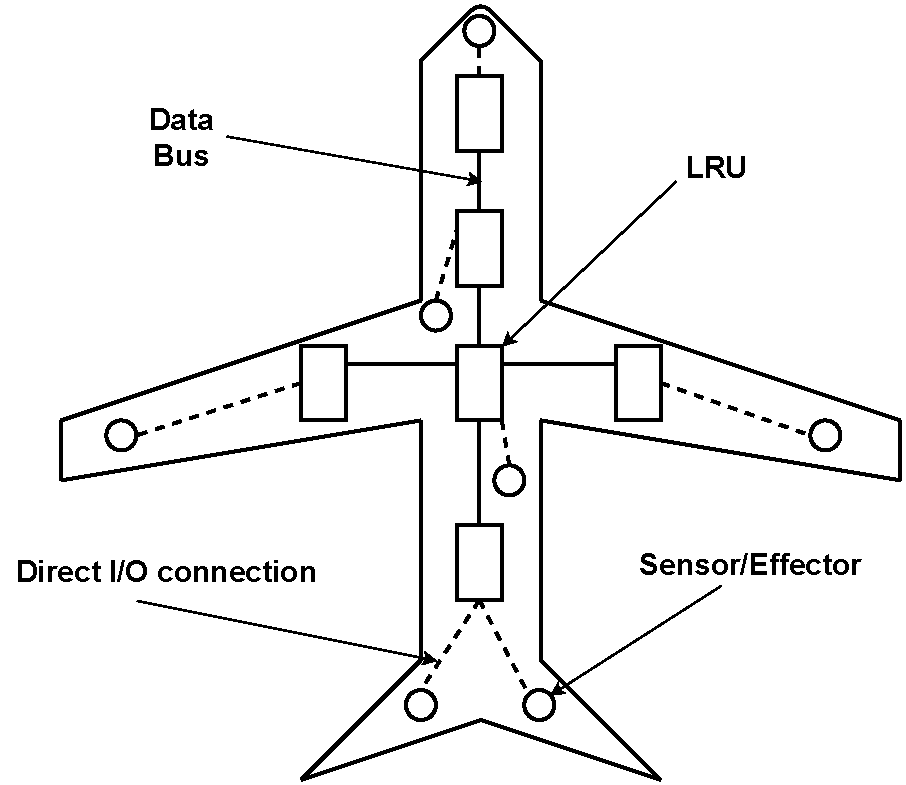
\includegraphics[width=1.0\textwidth]{figures/federated_architecture.pdf}
    \caption{Simplified visualization of the federated avionics architecture, showing \gls{lru}, sensors, effectors, and the global data bus}\label{fig:federated_architecture}
\end{figure}
\begin{figure}
    \centering
    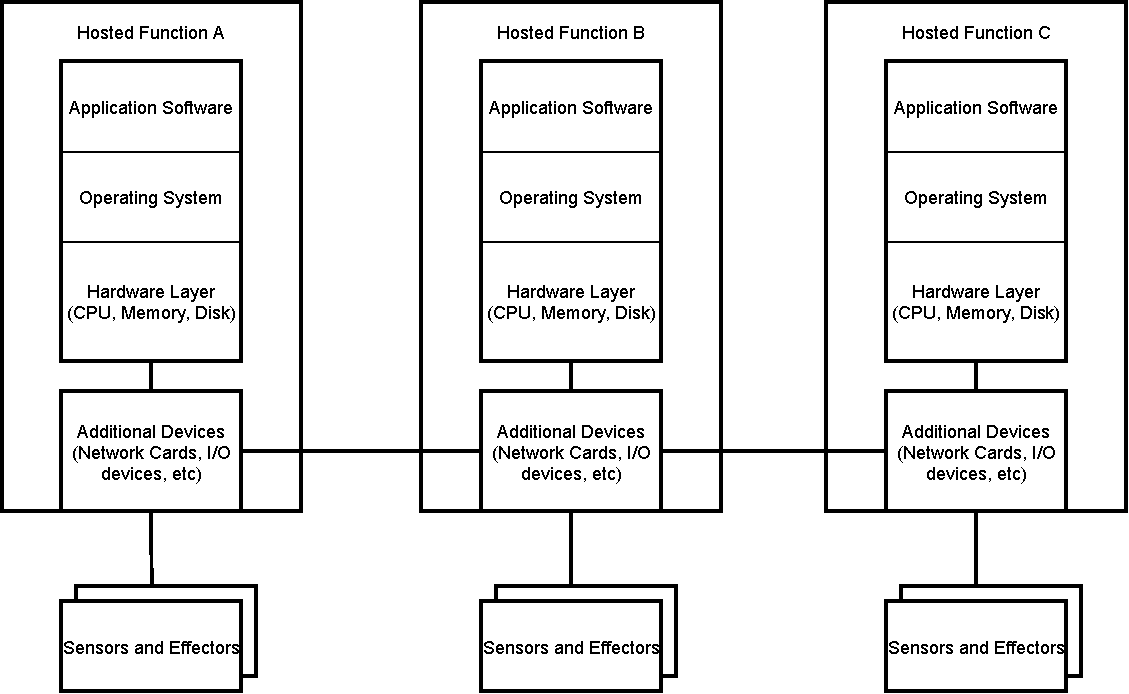
\includegraphics[width=1.0\textwidth]{figures/federated_architecture_components.pdf}
    \caption{Internal system architecture and interaction between \glspl{lru}}\label{fig:federated_architecture_components}
\end{figure}

\section{Integrated Modular Avionics}\label{section:integrated_modular_avionics}
\glsfirst{ima} is the direct successor of the federated avionics architecture. The idea behind \gls{ima}
is to consolidate the distributed hardware in one central flight cabinet. A Flight cabinet is very similar
to a rack in a datacenter. They can host multiple processing units, each comes with its own hardware stack
consisting of a \gls{cpu}, \gls{ram}, disk space and connectors for input and output\cite{prisaznuk1992integrated}. These servers are then plugged-in 
into the flight cabinet. Each server can host more than one avionic function and each function is allocated on partitions.
Partitions can be created on different ways and has been standardized in \gls{arinc653}\cite{vanderleest2010arinc}. The most common approach
is the use of a hypervisor (how this is implemented is being discussed in \autoref{section:workload_partitioning_strategies}). 
The flight cabinet provides power and required network connection to the plane's global data bus
as described in \gls{arinc629}\cite{isik2010arinc} or \gls{arinc429}\cite{fuchs2012evolution}. \gls{arinc629} is the successor of the data bus \gls{arinc429}.
Effectors and sensors communicate with the flight cabinet over \gls{arinc629}\cite{prisaznuk1992integrated}.
Sensors or effectors that are incompatible with \gls{arinc629} may communicate over remote data concentrators. Remote data concentrators are gathering data from sensors
or sending data to effectors over traditional \gls{io} connections. The gathered data or the received actions are communicated via \gls{arinc629} or \gls{arinc429}. Therefore,
remote data concentrators act as bridges between such devices and the data bus.
Using a central flight cabinet cannot replace all \glspl{lru} in the plane\cite{watkins2007transitioning}. These \glspl{lru} needs to be either integrated into the flight cabinet
or connected to the global data bus, for example via remote data concentrators. \autoref{fig:ima} depicts a simplified view on integrated modular avionics architecture in a plane.
The number of \glspl{lru} has been reduced and one central flight cabinet has been introduced. Remote data concentrators are working as bridges between sensors and effectors incompatible
with the data bus standard and the hosted functions in the flight cabinet. \autoref{fig:ima_components} shows the modules inside of such a flight cabinet. The flight cabinet
possesses multiple processing units. Each processing unit is comparable to a dedicated computer with its own hardware and operating system. These processing units
are being connected via a network layer and each processing unit hosts one or more hosted functions. Hosted functions are isolated from each other and have
a fixed predetermined set of resources and execution time.

\begin{figure}
    \centering
    \includegraphics[width=1.0\textwidth]{figures/ima.pdf}
    \caption{Simplified visualization of the integrated modular avionics architecture, showing sensors, effectors, cabinets and the data bus \glspl{lru}}\label{fig:ima}
\end{figure}

\begin{figure}
    \centering
    \includegraphics[width=1.0\textwidth]{figures/ima_components.pdf}
    \caption{View into a flight cabinet}\label{fig:ima_components}
\end{figure}

This system architecture has numerous advantages over the federated avionics architecture. Due to the more centralized approach \gls{ima}
is able to reduce weight via better cable management and less distributed processing units. Computing resources can be used more efficiently
via hosting multiple avionics functions on one processing unit. This leads to a higher system saturation. A positive side effect is less
energy consumption and a smaller ecological footprint. The reduced weight creates more space for cargo, fuel or passengers. 
Hardware consolidation leads to a consolidation of development efforts, which achieves cost and time savings\cite{watkins2007transitioning}.
The common processor allows the developer to focus on the hosted avionic function, enabling a better development experience and less error-prone
flight software. Separating software and hardware is a benefit during the certification process, because the certifying authority can certify
software and hardware separately. This has just another huge impact on cost and time savings. Additionally, upgrading the hosted function
becomes a lot easier, because of the hardware and software separation and less expensive hardware, due to standardized and more common
processing units. Another important benefit can be achieved via adopting the idea of open software and hardware. An open system architecture
with open standards can lead to a more competitive market due to industry-wide participation and exchangeability between hardware or
software applications. This way development and hardware costs can be reduced, because development cost gets distributed among all contributing
companies and mass production of standardized and open hardware shrinks marginal costs\cite{black2006open}. Moreover, the decoupling between hardware and software
can have a positive effect on new emerging companies, considering the lower costs\cite{watkins2007transitioning}. Software virtualization makes it easier to develop the
software, without buying expensive physical development kits. The software is being virtualized, tested and can be much later evaluated on real hardware, speeding up
the development process and time to market.

\section{Distributed Integrated Modular Avionics}\label{section:distributed_integrated_modular_avionics}
While \gls{ima} introduced a central architecture via consolidating computing resources into one central flight cabinet
\gls{dima} takes a different approach. \gls{ima} has shown that it is able to successfully reduce the number of components
in the plane with increasing number of hosted functions, because of its shared hosting infrastructure\cite{fuchsen2009preparing}.
Although this had positive effects on weight and cost management, there is room to improve in form of cable management.
Due to the centralized architecture it is necessary to connect every sensor and effector in the plane with the central flight cabinet
in the fuselage\cite{mccabe2009avionics}. This possible increase of cable length can be prevented via using ideas from the federated avionics and \gls{ima}.
\gls{dima} suggests a distribution of processing units, while taking into account the advantages of a central flight cabinet.
Instead of one central flight cabinet it is possible to redistribute the avionics functions over multiple flight cabinets distributed
in the plane's fuselage (see also \autoref{fig:dima}). This way it is possible to successfully exploit the advantages of the integrated architecture, while achieving
further improvements in the cable management\cite{li2012avionics}. Cable management is not the only possible adjustment for improvement.
The commercial cloud computing industry experienced a huge success over the last couple of years and these achievements can be used
for creating synergies between these two areas and applying cloud computing ideas in \gls{dima}. According to the \gls{nist} cloud computing is defined as:
\begin{displayquote}
\enquote{Cloud computing is a model for enabling ubiquitous, convenient, on-demand network access to a shared
pool of configurable computing resources (e.g., networks, servers, storage, applications, and services) that
can be rapidly provisioned and released with minimal management effort or service provider interaction.}\cite{mell2011sp}
\end{displayquote}
Although not all aspects of cloud computing are applicable on aviation, some of these aspects are.
One of these aspects is the separation into different service layers:
\begin{itemize}
    \item \gls{saas}
    \item \gls{paas}
    \item \gls{iaas}
\end{itemize}
\gls{saas} is handling all applications. \gls{paas} is responsible for the platform, where these applications
are running on (for example a hypervisor or services like webserver or databases). \gls{iaas} is the underlying
infrastructure (server, storages, networking). These three layers can be mirrored on the aviation world as follows:
\begin{itemize}
    \item \gls{saas}: Hosted functions
    \item \gls{paas}: The virtualized processing units or separation kernels
    \item \gls{iaas}: flight cabinets, remote data concentrators, the plane's data bus
\end{itemize}
Via separating each of these layers the aviation industry gains stronger standardization, more reliability and more effective
development workflows. Instead of selling one big monolithic system, separating makes it possible to develop products
for specific layers and interconnect them with the other layer via standards. These standards can be, as shown in \autoref{section:integrated_modular_avionics},
drivers for competition and exchangeability. Another aspect of cloud computing is the free and configurable allocation of applications\cite{li2012avionics}.
Dedicated storage, processor or sensor clusters would allow on-demand access from applications. Nevertheless it is a challenge to make this access reliable
and safe. Furthermore using standardized software may allow
interconnection between the plane and ground units (for example: real-time weather data transmitted from the ground to the plane).
This is partly comparable to the tactical data link of military units that get real-time radar data on their \gls{hsd}.

\begin{figure}
    \centering
    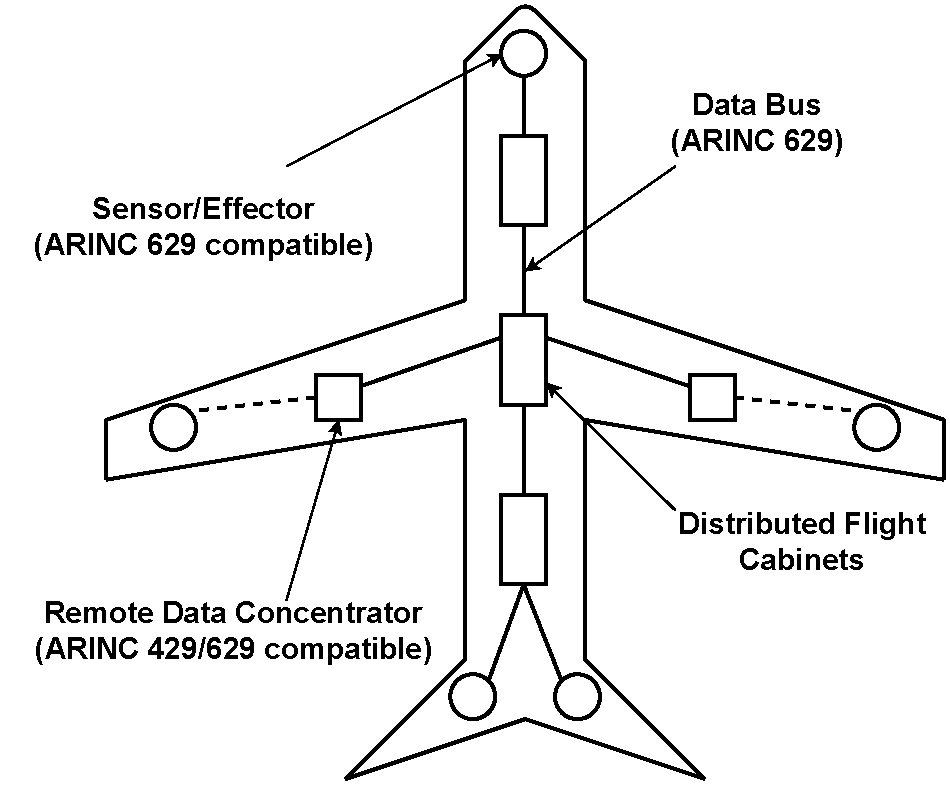
\includegraphics[width=1.0\textwidth]{figures/dima.pdf}
    \caption{Visualization of distributed flight cabinets}\label{fig:dima}
\end{figure}

\section{Workload Partitioning Strategies}\label{section:workload_partitioning_strategies}
Planes are composed of complex distributed systems with different tasks, requirements and environmental influences.
Every system has its own set of risks and possible impacts.
These different risks are known as \gls{dal} or \gls{idal} and have been defined
in the \gls{arp4754} as follows\cite{arp4754a2010guidelines}:
\begin{description}
    \item[A] Catastrophic system failures
    \item[B] Hazardous system failures
    \item[C] Major system failures
    \item[D] Minor system failures
    \item[E] No safety effect    
\end{description}

Due to these different risk levels it becomes important to isolate systems from each other. A system
with a low risk level should never have direct nor indirect impact on another system. In conclusion
the following measures are necessary to satisfy the safety and security requirements in planes:

\begin{itemize}
    \item Reserved \gls{cpu} time
    \item Reserved memory
    \item Reserved disk space
    \item \gls{qos}
    \item Network isolation
    \item Process isolation
    \item Privilege dropping
\end{itemize}

Reserved \gls{cpu} time means that every task has a strict time partition to work with.
Normally, cpu time is being shared on single processor systems. The operating systems simulates
parallelism via fast context switches. Multiple tasks are being executed consecutively switching
between them. This creates the impression that the system behaves parallel, but in reality it does not.
On multi processor systems real parallelism is possible. Reserved memory refers to a fixed memory
partition in the \gls{ram}. Reserved disk space refers to guaranteed space on a hard disk for storing
persistent data. Network isolation and Process isolation ensures a noisefree and secure runtime environment.
Processes should not be disturbed by other processes either on process or network level. Furthermore,
each process has to drop privileges. Dropping privileges increases the safety and security of a service,
because it is less likely to interfere with other processes if the process has no privileges to do so.
\gls{qos} gives certain processes with higher importance or risk level a higher priority. For example,
a system that controls the radar should have a higher priority than a system that just controls
the ambient lights in the passenger cabin.
Many of the above mentioned measures reveal other measures as direct dependencies. For example,
it is not possible to do proper \gls{qos} without an observable system that gets properly monitored.
Another example is the importance of security. On the first view security might be untangled of safety,
but in reality safety and security have a direct effect on each other. If the system is insecure it cannot
be safe and reliable, because every possible security incident could undermine all reliability promises.
The same applies to safety. An unsafe and unstable system cannot be considered secure, because these
weak points in the reliability might weaken the security. Just imagine a system that controls
permissions or security related functions. The system itself may be secure, but if it is unreliable 
it may has a direct effect on the security of other systems that depend on this particular system.
Additionally, planes have further constraints and requirements on software. One of these requirements
is a guarantee on response. Certain software systems in planes must respond before a given deadline.
This is called real-time communication. Real-time communication breaks down into the following types\cite{worn2006echtzeitsysteme}:

\begin{description}
    \item[Hard] The system has to satisfy all constraints. Responses are always on time. If a response would come too late it would inflict damage.
    \item[Firm] Executed tasks are worthless when their response does not satisfy the time constraint. No damage happens.
    \item[Soft] There are time constraints for requests and responses, but a tolerance exist. Delays are acceptable (as long as they fit in a specific time frame).
\end{description}

With all of these requirements it is obvious that there need to be technical implementations to satisfy all constraints.
The real-time constraints can be satisified via implementing real-time capabilities on operating system or kernel level.
Prominent examples are VxWorks' real-time operating system\cite{vxworks}, FreeRTOS\cite{freertos} or the real-time patches for the linux kernel\cite{realtimelinux}.
All other requirements are being solved either via virtualization or via containerization. There are two types of virtualization: Full virtualization and paravirtualization.
While full virtualization creates an almost full virtualized hardware including virtualized memory or \gls{io} devices, the paravirtualization does only virtualize
the software layer. The hardware stack will not be virtualized. Although this approach increases performance it is considered as less secure. With virtualization
it is possible to successfully isolate processes from each other and provide a dedicated workload partition for a specific software with its own \gls{ram} and \gls{cpu}.
The key element in this approach is the hypervisor. The hypervisor is the abstraction layer between the hardware, the software and their virtualized counterpart. 
Type 1 hypervisors run directly on the hardware, while type 2 hypervisors are running
on a dedicated host OS. Both hypervisors can usually virtualize a finite number of guests (finite, because the hardware resources are finite). Guests can be either applications or whole operating systems.
Many hardware provide direct support for virtualization, such as special instruction sets for \glspl{cpu}.
Containerization uses operating system or kernel level features to isolate processes or resources. In the Linux kernel this usually works via
making use of namespaces, kernel capabilities, control groups, union file systems and additional kernel features such like the \gls{ebpf}. Linux namespaces have been heavily influenced by namespaces in Plan 9 (an alternative
operating system by Bell Labs) and zones in Solaris. Contrary to traditional virtualization, namespaces do not need a hypervisor layer, instead the kernel offers
a single system call called \emph{setns()}\cite{mannamespaces}. The Linux namespace \gls{api} consists of six dedicated namespaces, each responsible for a different isolation environment\cite{namespacelist}:
\begin{description}
    \item[mnt] responsible for filesystem mount points
    \item[pid] responsible for processes
    \item[net] responsible for the network stack
    \item[ipc] responsible for \gls{ipc}
    \item[uts] responsible for \gls{uts}
    \item[user] responsible for \glspl{uid}
    \item[cgroup] responsible for \glspl{cgroup}
    \item[time] responsible for time  
\end{description}
The first namespace \emph{mnt} specifies the filesystem hierarchy for the isolated process or a group of processes. With this namespace it is possible
to mount only a specific directory structure into the isolated environment. This ensures that a process from environment \emph{A} cannot
access files on the host system or in another environment. The \emph{mnt} namespace has become especially useful in combination with union file systems.
Union file systems are layered filesystems and allow to mount multiple directory structures over each other. Docker uses this technology for combining
different layers to a full Docker container image. The second namespace \emph{pid} gives the system the opportunity to run multiple processes 
with the same \glspl{pid} on the host system. Running multiple processes with the same \gls{pid} on one system fulfills different purposes.
On one hand this provides reliability across different hosts. Via this approach it is possible to run a process with the same \gls{pid} in different
environments on different physical hosts. On the other hand it provides isolation. The process can only see other processes contained in the same namespace\cite{lwnnamespace}.
The \emph{net} namespace is responsible for everything network related. It provides the isolated environment with \gls{ip} addresses, ports, routing tables
and virtual network devices. \emph{net} is mostly being used for isolating network connections from each other. For example a namespace \emph{A} could provide
its own ports and internal IP addresses, while a namespace \emph{B} could provide the same port. The ports can be forwarded to the host via port-forwarding.
The \emph{ipc} namespace handles everything \glsfirst{ipc} related (message queues, Linux signals like \emph{sigkill} for killing processes etc).
For dealing with different hostnames in different namespaces the \emph{uts} namespace is being used. The last three namespaces implemented by Linux
are the \emph{user}, \emph{cgroup} and \emph{time} namespaces. \emph{user} is responsible for \glsfirstplural{uid} and \glsfirstplural{gid}. With
the namespace \emph{user} it is possible to differentiate users or groups with the same \glsplural{uid} or \glsplural{gid} in different environment.
For example, having the \emph{root} user (the administrator account on Linux systems) in different isolated environments. The user \emph{root}
is identified by the \gls{uid} 0 and the \gls{gid} 0. Different times in isolated environments are provided by the \emph{time} namespace.
The last namespace, the \emph{cgroup} namespace, is responsible for the \glsfirstplural{cgroup}. A \gls{cgroup} enables the system to limit
and monitor resources inside of a namespace via providing a pseudo-filesystem called cgroupfs\cite{mancgroups}. Each \gls{cgroup} consists
of one or more processes and each process is being modified by a subsystem (also known as resource controller). Subsystems work as modifiers
for these processes. Via these modifiers it is possible to set specific limits or monitor the processes. For example, limiting the available
\gls{cpu} time or memory for a process, increasing the priority for network traffic, limiting access to \gls{io} devices or
monitoring events created by a process\cite{mancgroups}. The last two missing building blocks for secure containers are kernel capabilities and the \glsfirst{ebpf}.
Kernel capabilities provide a more granular access to kernel features such like mounting or creating ports\cite{dockersecurity}.
Common kernel capabilities are \emph{CAP\_CHOWN} (changing the owner and group of a file), \emph{CAP\_NET\_BIND\_SERVICE} (allow the binding of ports under 1024), 
\emph{CAP\_SYS\_ADMIN} (allow system administrator access), \emph{CAP\_NET\_ADMIN} (allow network administrator access, a complete list can be found
in the corresponding man page for kernel capabilities\cite{mancapabilities}). The \glsfirst{ebpf} is the successor of the \glsfirst{bpf}. The \gls{bpf} is 
well known for its human readable filtering language that allows filtering, monitoring and analyzing packets in computer networks. Core of the \gls{bpf}
is a \gls{jit} compiler that translates the human readable \gls{bpf} language into machine readable byte code. Contrary to its predecessor, \gls{ebpf} is not limited
to network packets. With Linux version 3.18, \gls{ebpf} has been embedded into the Linux kernel as virtual machine and allows filtering for any sort of \glsfirst{ipc},
such like socket connections, system calls (syscalls) or kernel permission delegations. \autoref{fig:workloads} gives an overview over different workload partitioning and
deployment techniques. On the far left is the traditional setup with the hardware, an operating system running on the hardware, the applications and their shared libraries.
The second pillar shows a type 2 hypervisor with a hardware, an operating system, shared libraries on the operating system, a hypervisor and virtual machines. Each virtual machine
comes with their own operating system, shared libraries and the actual payload (the application with the workload). The type 1 hypervisor simplifies this setup with running
a hypervisor directly on the hardware. In this case, the hypervisor is hypervisor and operating system at once. The container deployment comes with the hardware, an operating system 
and its shared libraries and a container runtime. Each container can consist of different parts. A container can consist of only one static built executable or an application and shared libraries.
Shared libraries minimize the size of software via sharing common methods, for instance a library for \glsfirst{rpc} or \gls{dns} lookups. When the executable has been linked dynamically,
the executable can dynamically look up these common methods.
Contrary to dynamic linking is static linking, where a software is being compiled with all its dependencies into one executable. Although all deployment techniques may look similar at a first glimpse,
they are indeed completely different. A virtual machine allows stricter isolation compared to running all applications without virtualization and a container can consist of a single binary.
\begin{figure}
    \centering
    \includegraphics[width=1.0\textwidth]{figures/workloads.pdf}
    \caption{Overview over different workload partitioning and deployment techniques}\label{fig:workloads}
\end{figure}

\section{Challenges and Opportunities}\label{section:Challenges_And_Opportunities}
Prior, this thesis has explored past, present and future avionic system architectures. On the next pages it is going to examine
challenges in these avionic system architecture designs and possible enhancements in the avionic domain in general. This document is explicitly ignoring the certification
process of software. It is known that a certification process in the avionic domain can be slowly and very costly, due to its
high risk to passengers, flight personnel and civilians on the ground. Enhancing this certification process via altering the certification itself, while matching the right balance between safety
and development speed or costs, is explicitly not topic of this research. Instead, this document tries to focus on few main questions.
The first identified challenge is the increase of development speed in the avionic domain. Pushing innovations and new technologies fast is a major
success factor. Maintaining a hardware and software stack for a traditional avionic system architecture, like the federated architecture, is a
huge cost and time disadvantage. The developer cannot use the standard development tools and needs to adapt to the new environment. Moreover,
buying the necessary equipment and constantly adjusting the software to this equipment are toilsome and complicated. Every hour of additional
work is a cost factor that leads to higher unit prices, smaller profit margins and less time for more features. Costs directly lead to the next
challenge: Decreasing development costs and increasing feature output. Considering the tight entanglement of soft- and hardware in federated systems
these stacks become very cost intensive. Also, the feature output is limited to the required hard- and software,
hence limiting possible performance or functionality gains. Performance is another challenge. As a result of heavy use of virtual machines the performance
gains are not as high as they could be. The hard- and software limitations make the system less extensible and less adjustable. Another challenge is the
proprietary avionic system development environment. Proprietary standards, hardware- and software have devastating effects on innovation, safety, security,
costs and technological development. Innovation is affected negatively, because of less communication between companies. Open architectures, software or hardware
increase communication and share knowledge between all development entities. These shared knowledge and improved communication is known for increasing
security of software\cite{hoepman2007increased}. Restricting access to the source code may help restricting the attacker's knowledge for executing attacks, but it is shown that
``keeping the source code closed appears to be difficult''\cite{mercuri2003security}. Furthermore, patches for open source software are released twice as fast
as for closed source software\cite{witten2001does}. The increased pace of patching the software underlines the increased development speed and its connected
benefits. Many of the highlighted challenges are not new for the tech industry. The cloud industry has solved several of these challenges successfully.

\chapter{Cloud-Native}\label{chapter:cloud_native}
\section{Introduction}
Containers are not a new concept. The idea behind them goes back to systems like Solaris, FreeBSD or Linux. FreeBSD has released their first container-alike
isolation environment, called \emph{jails}, in 2000\cite{FreeBSD4Announcement}. Jails are heavily being influenced by the chroot system call on Unix systems.
The chroot system call has been introduced with Version 7 Unix in 1979\cite{BYTE}. The concept has been there all the time so what was missing?
Although containers were in use by system administrators the workflow was not developer friendly enough. Big companies like Google
realized the potential of containers early and started to heavily use them in their own infrastructure, but the overall success
came with open source technologies like Docker or Kubernetes. It turned out that opening up the development process of these technologies
has been the perfect foundation for creating a community that spans over several companies and industry branches. This community is under
supervision of the Linux Foundation and is called \glsfirst{cncf}\cite{CNCFFounding}. The \gls{cncf} built an enormous ecosystem for
running and orchestrating containers. \autoref{fig:landscape} visualizes the scale of the \gls{cncf} related projects\cite{CNCFLandscape}. Considering that
that the \gls{cncf} was founded in 2015 this is clearly a huge success for the containerization of applications in different industry branches, especially
for the cloud computing industry. Looking at the landscape it can be seen that the \gls{cncf} covers different areas and expands wide beyond containerization.
Just to name a few different areas and their sub areas on the landscape:

\begin{description}
    \item[App Definition and Development] databases, streaming and messaging, application definition and image build, continuous integration and delivery
    \item[Orchestration and Management] scheduling and orchestration, coordination and service discovery, remote procedure call, service proxy, api gateway, service mesh
    \item[Runtime] Cloud-Native storage, container runtime, Cloud-Native network
    \item[Provisioning] automation and configuration, container registry, security and compliance, key management
    \item[Observability] monitoring, logging, tracing, chaos engineering
\end{description}

While some of the above areas play only a minor role in the aviation industry some areas are usable or will play a bigger role in the future.
Especially, areas like scheduling and orchestration or container runtime are of interests for the aviation industry, because
these areas provide related functionality compared to current solutions in actual use within the aviation industry.

\begin{figure}[H]
    \centering
    \includegraphics[width=1.0\textwidth]{figures/landscape.png}
    \caption{Cloud-Native Computing Foundation Landscape}\label{fig:landscape}
\end{figure}
 
\section{Docker}
Docker (released in 2013\cite{DockerRelease}) has revolutionized the way containers are being used.
Before Docker, the primary users of containers have been sysadmins, who used containerization to isolate environments from each other. With Docker
this workflow has changed. Docker has introduced a unique file format, called Dockerfile, for describing a container consisting of different layers. These layers
are stacked on each other, with the help of union file systems, for a final Docker image. This process has a few advantages. Each layer can be cached separately, leading
to less disk usage and faster container build times. Layers do not need to be from the same author. In Docker it is very common to re-use common Docker images
as a base layer and add additional payload to them via adding layers on top of the base layer. The base layer is often called the base image and the most popular
base image is the \emph{scratch} image. \emph{Scratch} is just an empty Docker layer. All other base images use the \emph{scratch} image as start point for the build process.
Base images can be whole Linux distributions like Debian, proprietary operating systems from the industry or just a directory structure. For example, Google provides
a \emph{distroless} Docker image that just contains time zone data and the global certificate chain\cite{Distroless}. The \emph{distroless} image is mainly in use for shipping
static binaries inside of Docker. This is common practice for languages like Rust or Go. Shipping just the binary leads to a much smaller attack surface. Having no shell inside
of the image makes it impossible for an attacker to gain shell access to such a container and missing additional executables make it difficult to
exploit additional executables for building an attack chain (for example via using network utilities for opening a reverse shell into the container).
\autoref{lst:dockerfile} shows an example multi-stage Dockerfile with different layers. Each line in the file is a separate layer in the final image
and each \emph{FROM} statement defines a different stage in the Docker image build process. In the first stage of the Dockerfile
a small hello world program will be written in the programming language Go (often referred to as Golang) and compiled. In the second stage,
the executable from the first stage will be copied to the new second stage, placing it into a \emph{distroless} image for reducing the possible
attack surface and making the executable available for further distribution as Docker image. The first stage starts with the statement
\emph{FROM docker.io/golang:1.17 AS GO\_BUILD}, setting the base image to \emph{golang} with version 1.17 from the Docker registry \emph{docker.io}
and naming this stage \emph{GO\_BUILD}. A Docker registry is a public or private repository for Docker images. 
The second statement \emph{WORKDIR /go/src/app} sets the working directory for the build process. It is comparable to moving to a folder
in a Windows system or changing the directory in a Linux system via the command line command \emph{cd}. The next three statements starting
with \emph{ENV} are setting environment variables. Environment variables are an operating system feature for setting variables outside
of programs for configuration purposes. \emph{GOOS} sets the target operating system to Linux, \emph{GOARCH} sets the architecture to amd64
and \emph{CGO\_ENABLED} disables the libc support for the Go build process. Disabling the libc support is equal to disabling linking
to shared libraries, resulting to a static compiled binary that can be moved on different systems as long as the target operating system
and architecture stays the same. With the next three \emph{RUN} statement it is possible to execute commands in the base image
\emph{docker.io/golang:1.17} (this also means that our base image is actually based on Linux). The \emph{echo} command
prints our Go hello world code and pipes it into a file called \emph{main.go}. Using \emph{go mod init app} initializes
the Go build and dependency system with a name for the app. Running \emph{go build -o /out/app .} will build the \emph{main.go}
file in the current directory and move the created executable \emph{app} to the directory \emph{/out/}. Using the next
\emph{FROM gcr.io/distroless/base} statement a new stage will be build with a new base image for the final image holding the executable
and reducing possible attack surface by utilizing Google's \emph{distroless} images. The \emph{COPY} statement will
copy the built executable from the first stage into the new second stage and the \emph{ENTRYPOINT} statement will set
the path of the application as entrypoint for the container startup. It is important to differ between images and containers.
Containers are running instances of images. The entrypoint is the start point from each container and be compared to the main function
of most C-alike programming languages or the init system of a modern operating system. \autoref{lst:dockerbuild} shows
the output of building the Docker image. Each step is equal to one layer of the final image and each layer has a unique
\gls{sha256} checksum over the binary content of the layer for ensuring integrity and reproducibility. This minor information
has a unique impact on supply chain security, developer experience and costs, because with each layer cryptographically
identified it is much more difficult to tamper with the build process, allowing secure access to cached layers
and leading to faster development speed and lower costs. The final image can be run as container via executing
\emph{docker run} leading to the promised \emph{Hello World!} line. 
\begin{minipage}{\linewidth}
\begin{lstlisting}[caption={A multi stage Dockerfile with different layers},label={lst:dockerfile}]
FROM docker.io/golang:1.17 AS GO_BUILD
WORKDIR /go/src/app
ENV GOOS=linux
ENV GOARCH=amd64
ENV CGO_ENABLED=0
RUN echo "package main\nimport \"fmt\"\nfunc main() { fmt.Println(\"Hello world!\") }" > main.go
RUN go mod init app
RUN go build -o /out/app .

FROM gcr.io/distroless/base
COPY --from=GO_BUILD /out/app .
ENTRYPOINT ["./app"]
\end{lstlisting}
\end{minipage}
\begin{minipage}{\linewidth}
\begin{lstlisting}[caption={Output of a docker build run with shortened SHA256 checksums},label={lst:dockerbuild}]
STEP 1: FROM docker.io/golang:1.17 AS GO_BUILD
STEP 2: WORKDIR /go/src/app
--> Using cache baa3b5061ca
--> baa3b5061ca
STEP 3: ENV GOOS=linux
--> Using cache fe142d360ee
--> fe142d360ee
STEP 4: ENV GOARCH=amd64
--> Using cache 49771a6a4a6
--> 49771a6a4a6
STEP 5: ENV CGO_ENABLED=0
--> Using cache edf307d8374
--> edf307d8374
STEP 6: RUN echo "package main\nimport \"fmt\"\nfunc main() { fmt.Println(\"Hello world!\") }" > main.go
--> Using cache ca435b8adf9
--> ca435b8adf9
STEP 7: RUN go mod init app
--> Using cache 19b7a23f24d
--> 19b7a23f24d
STEP 8: RUN go build -o /out/app .
--> Using cache baeee09e19f
--> baeee09e19f
STEP 9: FROM gcr.io/distroless/base
STEP 10: COPY --from=GO_BUILD /out/app .
--> Using cache 5ab01f9acf7
--> 5ab01f9acf7
STEP 11: ENTRYPOINT ["./app"]
--> Using cache 288ac81c34b
--> 288ac81c34b
\end{lstlisting}
\end{minipage}
\section{Open Container Initiative}
In June 2015 leading container projects, such like Docker and CoreOS (a minimal Linux distribution for running containers), launched the \gls{oci}
under auspices of the Linux Foundation\cite{OCIabout}. The \gls{oci}'s purpose is the standardization of Docker's container image specification (image-spec\cite{ImageSpec}), container runtime (runtime-spec\cite{RuntimeSpec})
and content distribution (distribution-spec\cite{DistributionSpec}). These three specifications address everything from building a container image, distributing the image
over a container registry, and running the container. Standardization enables interchangeability of all three implementations and increases possibilities for their production usage.
In the following, this thesis will have a short glimpse on each of the specifications. A full writeup would break the constraints of this thesis. It is recommended to read
the original specification, if more information is needed. The image specification has five essential components:

\begin{description}
    \item[manifest] provides a set of layers and a configuration for a specific image runnable on a specific architecture and operating system
    \item[image index] provides a set of manifests with different architectures and operating systems
    \item[image layout] provides a file system layout (the contents of the image) 
    \item[filesystem layers] provides information about merging different layers to one image
    \item[configuration] provides the configuration of the image, provided by the Dockerfile (environment variables, entrypoints, etc)
\end{description}

\autoref{lst:imageManifest} depicts a very simplified example image manifest. The \gls{sha256} checksums have been shortened for saving space in this document.
The manifest shows the schema version, a configuration, multiple layers and annotations. The configurations and layers have media types, a field for the
size and a digest (a checksum) of the addressable content. Annotations provide further information for the image. The \gls{oci} manifest specification
defines a few predefined annotations, but at last these are just customizable strings. Annotations allow additional metadata for images, thus
providing information for various other use cases, like easier search in an \gls{oci} compatible registry or information about its maintainers.
With the manifest it is possible to address the content via its offset and to provide integrity via digests \cite{ImageManifestSpec}. One or more image manifests can form
an image index. An image index is a set of different image manifests for different operating systems and architectures \cite{ImageIndexSpec}. \autoref{lst:imageIndex} illustrates
such an image index with support for two platforms. The first addressed manifest links to a manifest for MacOS with M1 chipset. The second addressed manifest
refers to a manifest for Linux with amd64 chipset. Furthermore, it is possible to add additional annotations to the image index definition. As mentioned earlier,
an \gls{oci} image consists of different layers. These layers are defined in the image layout and the filesystem layers specifications. One or more compressed layers are applied
on top of each other to create the entire root filesystem of the image\cite{ImageFSSpec}. The filesystem layers specification can handle 
additions, modifications and removals of various file types, such like directories, sockets, symbolic links, block devices, or regular files\cite{ImageFSSpec}.
All of these layers are described as an image layout. Each layer is stored in the image layout as \gls{blob} and addressable via its \gls{sha256} digest. An \gls{oci} image layout
is comparable to a directory in a filesystem. A \gls{blob} directory stores all layers, an index.json file provides platform interoperability via establishing the relationship
between each layer and their target platform \cite{ImageLayoutSpec}. \gls{oci} layout files work as marker and version identifier of the \gls{oci} layout. While the prior mentioned specifications
define the structure of the \gls{oci} image, the configuration specifies the environments, entrypoints, volumes, working directory, commands that should be executed and other configuration parameters.
The \emph{docker image inspect <docker image>} command prints a full OCI image configuration for a given image. \autoref{lst:imageConfiguration} shows the output of this command
for the prior mentioned OCI image, built from \autoref{lst:dockerfile}. The output has been cut down to the most important parts. Clearly visible is the environment in form of environment
variables, the command, the working directory, an entrypoint, the Docker version, a build date and the root file system layers. If compared with \autoref{lst:dockerfile} the similarities are obvious. 
This image configuration works as interface for the runtime specification. The \gls{cri} provides an interface for running \gls{oci} compatible images. Common implementations of the \gls{cri} are
Docker, Containerd\cite{Containerd} or cri-o\cite{CRIO}. Containers are encoded as filesystem bundles. A filesystem bundle consists of the container configuration as specified in the \gls{oci} image specification
and the container's root filesystem (referenced in the image configuration)\cite{FilesystemBundle}. These filesystem bundles are executed by the container runtime. The container runtime manages the state and the lifecycle
of the container. Every container runtime implementation must fulfil the \gls{cri} specification's lifecycle operations and commands for basic runtime interaction (create, start, stop, kill, etc).
Distributing a container image is described by the \gls{oci} distribution specification. The distribution specification defines all necessary components of an \gls{oci} image compatible registry
and its basic operations. Described are the pull of an image (the act of downloading \glspl{blob} and manifests from the registry), the push of an image (the act of uploading \glspl{blob} and manifests to the registry),
and the registry itself. 

\begin{minipage}{\linewidth}
\begin{lstlisting}[caption={An OCI image manifest with two layers, shortened sha256 checksums and two annotations},label={lst:imageManifest}]
{
    "schemaVersion": 2,
    "config": {
        "mediaType": "application/vnd.oci.image.config.v1+json",
        "size": 8652,
        "digest": "sha256:b5bb9d8014a0f..."
    },
    "layers": [
        {
            "mediaType": "application/vnd.oci.image.layer.v1.tar+gzip",
            "size": 40270,
            "digest": "sha256:c739918a22764..."
        },
        {
            "mediaType": "application/vnd.oci.image.layer.v1.tar+gzip",
            "size": 14743,
            "digest": "sha256:9f767b0b078d2..."
        }
    ],
    "annotations": {
        "org.opencontainers.image.authors": "Christian Rebischke",
        "org.opencontainers.image.title": "A very easy manifest example"
    }
}
\end{lstlisting}
\end{minipage}
\begin{minipage}{\linewidth}
\begin{lstlisting}[caption={An OCI image index with multiple manifests, shortened sha256 checksums and platform specifications},label={lst:imageIndex}]
{
    "schemaVersion": 2,
    "manifests": [
        {
            "mediaType": "application/vnd.oci.image.manifest.v1+json",
            "size": 9783,
            "digest": "sha256:6650b51fab815ad7fc331f...",
            "platform": {
                "architecture": "arm64",
                "os": "darwin"
            }
        },
        {
            "mediaType": "application/vnd.oci.image.manifest.v1+json",
            "size": 9543,
            "digest": "sha256:ed22e9fb1310cf6c2decab...",
            "platform": {
                "architecture": "amd64",
                "os": "linux"
            }
        }
    ],
    "annotations": {
        "org.opencontainers.image.created": "2021-12-19T16:39:57-08:00",
    }
}
\end{lstlisting}
\end{minipage}
\begin{minipage}{\linewidth}
\begin{lstlisting}[caption={An OCI image configuration created via docker image inspect (shortened)},label={lst:imageConfiguration}]
{
    "RepoTags": [
    "hello-world:latest"
    ],
    "Created": "2021-12-19T07:47:29.318765235Z",
    "ContainerConfig": {
    "Hostname": "motoko.shibumi.dev",
    "User": "0",
    "AttachStdin": false,
    "AttachStdout": false,
    "AttachStderr": false,
    "Tty": false,
    "Env": [
        "PATH=/usr/local/sbin:/usr/local/bin:/usr/sbin:/usr/bin:/sbin:/bin",
        "SSL_CERT_FILE=/etc/ssl/certs/ca-certificates.crt"
    ],
    "Cmd": [
        "/bin/sh",
        "-c",
        "#(nop) ",
        "ENTRYPOINT [\"./app\"]"
    ],
    "Image": "sha256:bc721b69a6af4bb...",
    "WorkingDir": "/",
    "Entrypoint": [
        "./app"
    ],
    "DockerVersion": "20.10.12",
    "Architecture": "amd64",
    "Os": "linux",
    "Size": 22013044,
    "VirtualSize": 22013044,
    "RootFS": {
    "Type": "layers",
    "Layers": [
        "sha256:c0d270ab7e0db0...",
        "sha256:e3d24823466584...",
        "sha256:589f2bccf144b2..."
    ]
    },
}
\end{lstlisting}
\end{minipage}


\section{Container Interfaces}
With the rise of the \glsfirst{oci}, more and more container management systems and orchestration services have been developed.
While the implementations of the \glsfirst{cri} provides basic runtime functionality for executing containers, it became clear that
an interface for running containers is not enough. The usecases for containers became more complex and orchestration services became
distributed over large network topologies. This distribution lead to the necessity of standardized networking and storage interfaces.
These interfaces are called \glsfirst{cni} and \glsfirst{csi}. This section summarizes both interfaces and gives a good introduction.
However, this section is not meant as complete guide for implementing these interfaces. \glspl{csi} provide an interface for new storage providers.
A storage provider is the vendor of the plugin implementation\cite{CSISpec}. Storage providers can be providers for local or remote storage.
Every local storage differs and there are different ways on a system to provide storage for an application. Local Storage can be offered
via device mappers, the \gls{lvm}, raw block devices, volume groups or many other operating system and hardware dependent systems. Remote
storage equally complicated with additional network capabilities and protocols, such like \gls{nfs} or ceph (the distributed, fault-tolerant storage platform).
Each of these storage providers have a different \gls{api} and different ways to read and write data on them.
Container orchestrators implement the \gls{csi}. Communication between the \gls{csi} plugin and the container orchestrator happens over \gls{rpc}. The most common \gls{rpc} protocol
in the cloud-native environment is \gls{grpc}. \gls{grpc} (invented in 2016 by Google) has the huge advantage that it is language independent, supports a very
simple service definition via Protocol Buffers and bi-directional streaming with several security features like authentication\cite{GRPCConcepts}.
Protocol Buffers is an \gls{idl}. \glspl{idl} offer a, for the developer, convenient way to describe an \gls{rpc} interface in a language independent and
human-readable way. \gls{grpc} and Protocol Buffers are the tools of choice for the \gls{csi}. The \gls{csi} presents basic functionality for 
dynamic provisioning of volumes (on-demand provisioning), attaching or detaching volumes, mounting or unmounting volumes from an orchestration node, creating or deleting snapshots
or provisioning new volumes\cite{CSISpec}. Snapshots are one-time states of a volume with data, they are not equal to backups. Snapshots allow the storage provider
to go back in time and restore data for a given time frame. For this operation the storage provider requires necessary metadata and a running service. This is what
distances them from a backup. A backup offers a reliable way to restore a full dataset in case of a disaster (for instance a hardware outage). A snapshot does not
offer this reliability and may fail if the underlying system is damaged. Usually, a storage provider implements an \glsfirst{api} that is \gls{csi} compatible
or a third-party implements a service that interprets the \glspl{api} of the storage provider plugin and translates it, to be \gls{csi} compliant. When container orchestrators
like Docker became distributed over multiple nodes the network became more relevant. The \glsfirst{cni} specification addresses this problem and proposes a standard interface
for enhanced network capabilities for future container runtime and container orchestration solutions. Equally to the \gls{csi} specification, the \gls{cni} specification is language agnostic,
but the reference implementation is written in Go\cite{CNISpec}. As of writing this thesis, there are already over 20 \gls{cni} compatible plugins from various cloud providers, hardware vendors
or third-parties. These plugin differ significantly, because they address different use cases, problems or network environments. The \gls{cni} specification abstracts these differences and provides
a common interface for all of them. \gls{cni} plugins are not bound to one specific layer of the \gls{osi}. For instance, the \gls{cni} plugin \emph{flannel} focuses on \gls{osi} layer 3 only, hence providing
every container with its own unique routable \gls{ip} address via spanning an IPv4 network over all container orchestration nodes in a cluster (a cluster is a group of multiple orchestration nodes, responsible
for running containers or managing the cluster)\cite{Flannel}. Other \gls{cni} plugins such like \emph{cilium} or \emph{calico} offer support for more \gls{osi} layers and more features, such like
traffic encryption, traffic monitoring, network policies or more graduated network and routing capabilities.

\section{Kubernetes}
\subsection{Introduction and History}
Although Docker has been released in 2013, Google has been using Containers for a much longer period of time. According to Google engineers, they are managing Linux containers at scale since
at least 2006\cite{burns2016borg}. This long history of Linux container management lead to several internal container orchestration platforms within Google, such like Borg\cite{verma2015large}, Omega\cite{schwarzkopf2013omega} or Kubernetes\cite{kubernetesWebsite}.
While Borg and Omega are internal projects and therefore proprietary, Kubernetes is open source and freely available on GitHub\cite{KubernetesGithub}. Since the Kubernetes release in 2014\cite{KubernetesFirstRelease}, Kubernetes has started a chain reaction
in the industry. More and more projects have been founded around Kubernetes as distributed container orchestrator. The \glsfirst{cncf} landscape lists a plethora of different projects and project domains around Kubernetes, such like continuous integration and continuous delivery frameworks,
service proxies, service meshes, Kubernetes compatible container runtimes, \glsfirst{cni} or \glsfirst{csi} plugins or security addons for Kubernetes. This extensibility is one of Kubernetes' many success drivers. Kubernetes offers everything necessary for running
\gls{oci} compatible containers distributed on one or more Linux hosts, called nodes. These \gls{oci} compatible containers do not even need to be containers in the traditional sense. It is possible, with a little bit of effort and the KubeVirt project\cite{KubeVirt},
to run small virtual machines with Kubernetes. Such virtualized containers are called microVMs. However, on default Kubernetes focuses on running containers as abstracted by namespaces, cgroups and other Linux kernel features. Kubernetes does this
slightly differently to other container orchestrators. The smallest manageable unit in the Kubernetes world is being called a \emph{pod}. A pod consists of one or more containers and possesses a few additional properties to enhance container management and orchestration.
These differences will be explained in more detail in the following sections.

\subsection{Architecture}
\begin{figure}[H]
    \centering
    \includegraphics[width=0.8\textwidth]{figures/kubernetes.pdf}
    \caption{Overview over a Kubernetes cluster with three control nodes and three worker nodes}\label{fig:kubernetes}
\end{figure}
In this section, this thesis explores the architecture of Kubernetes. \autoref{fig:kubernetes} depicts a Kubernetes cluster with three control nodes and three worker nodes. Many control nodes form a control plane.
Control nodes are responsible for managing the cluster, while worker nodes are carrying the actual application payload. In case of an airplane the worker nodes could, for example, carry applications for controlling
the cabin temperature, lights or the entertainment system. Each node is connected to each other via a reliable and highly available network plane (symbolized by a switch in the middle). All nodes consist of a
an operating system (Linux), a container runtime, a KubeProxy and a Kubelet. The operating system is very often a highly specialized Linux distribution, for instance Flatcar Linux\cite{FlatcarLinux} or Fedora's CoreOS\cite{FedoraCoreOS}.
Specialized Linux distributions have the huge advantage of being very minimal, high secure and require low maintenancy. They accomplish this via only shipping the Linux kernel, an init and service daemon like systemd\cite{systemd}
and a very small read-only base system. System upgrades are conducted through ostree image updates. The ostree is the operating system tree containing the base system. Contrary to other traditional Linux distributions like Debian,
these specialized Linux container operating systems do not update software independently. Instead, the system upgrade is conducted via upgrading the whole base system at once. This procedure allows a very high testability, reliability
and a lower maintenance compared to traditional Linux distributions. On top of the operating system is the container runtime, popular container runtimes are Containerd\cite{Containerd} or cri-o\cite{CRIO}. Docker was another famous
container runtime for Kubernetes clusters, but it got recently deprecated in favor of Containerd\cite{KubernetesDockerNews}. Other components of every cluster are the KubeProxy and the Kubelet. The Kubeproxy is responsible
for network connections between each node and establishes connections to each pod\cite{KubernetesComponents}. Kubelets are Kubernetes agents and are managing containers in each pod.
Additional components of a control node are an etcd\cite{etcd} instance, a Kube-Controller, a Kube-Scheduler and a KubeAPI instance. Etcd, is a highly available, reliable and distributed key-value store. Kubernetes uses etcd as its database for storing its actual 
and desired state. Every change on the Kubernetes cluster will be stored in the etcd cluster running distributed on all control nodes. Concensus is achieved via Raft, an advanced concensus algorithm proposed
by the Stanford University\cite{ongaro2013search}\cite{ongaro2014search}. Raft, that stands for replicant and fault-tolerant, implements consistency and partition tolerance as defined by Eric Brewer's CAP-theorem\cite{brewer2017spanner}.
Eric Brewer's CAP theorem states that a distributed system can only implement two of three properties of the CAP theorem. These three properties are consistency, availability and partition tolerance. Consistency is when each node
has the newest data, availability is when all read and write requests are always successful and partition tolerance means that the distributed continues to operate even when not all nodes are available\cite{bijlsma2020distributed}.
Raft guarantees consistency and partition tolerance, but it cannot guarantee availability due to unknown factors like network outages.  Instead of using time, Raft uses election terms and roles for each node. Everytime an election is held,
Raft will increment the term counter. On initialization all nodes have the role \emph{follower} and the term counter on each node is zero. The first election term begins with one follower nominating itself as \emph{candidate} and
advertising this nomination to all other nodes. The other nodes will react with an acknowledgement and the candidate node will be promoted to a \emph{leader}. The leader node sends heartbeats to every other node in the cluster.
When a cluster node receives such a heartbeat the node's timeout will be reset. As long as the leader stays healthy nothing happens and the cluster works as usual. As soon as the leader dies the other nodes will stop
receiving heartbeats. The missing heartbeart will lead to a timeout expiration. When this happens the expired node will increment the election term counter and nominate itself for a new leader and the process starts from new.
This process ensures the partition tolerance as defined by Eric Brewer's CAP theorem. Data can be added to the key-value store only through the leader node and all followers will forward write requests to the leader node. 
The message is considered committed as soon as the majority of nodes acknowledged the write operation. Read operations can be done on every node. This is equal to Eric Brewer's consistency property of the CAP theorem.
Further control node components are the Kube-Controller, the Kube-Scheduler and the KubeAPI. The KubeAPI provides an \glsfirst{api} endpoint for the cluster and external clients, for instance an admin who triggers changes on the cluster.
If a pod gets created the Kube-Scheduler will schedule the pod on a free node. Kubernetes supports different scheduling and rollout strategies for deployments. Finally, the Kube-Controller implements different processes for controlling
the cluster. For example, the Kube-Controller populates endpoints, takes care of service accounts, creates jobs or notices a node failure and responds accordingly\cite{KubernetesComponents}.
\subsection{Application Programming Interface (API) Overview}
One of Kubernetes' biggest success factors is its extensibility. Kubernetes provides a good maintained \glsfirst{api} and implements necessary interfaces for extending Kubernetes with functionality. In this section, this thesis
will highlight the most common \gls{api} resources in the Kubernetes \gls{api}, their purpose and their capabilities. For exploring the Kubernetes \gls{api} this thesis uses a single node cluster bootstrapped via Minikube\cite{Minikube}.
Minikube, written in Go, is a wrapper for bootstrapping a Kubernetes Cluster inside of one or more virtual machines. It allows a fast setup for local development and testing purposes, ideally for this thesis. Installing Minikube is rather easy:
One just have has to download Minikube from its official website and run the following command: \emph{minikube start --cpus 4 --memory 4096 --vm}. For running this command virtualbox is required as hypervisor. The command will download a slim
virtual machine, provision it with 4 \gls{cpu} cores and 4096 megabytes of \gls{ram}. The \emph{--vm} flag will choose the virtual machine backend type. Minikube is able to provision a Kubernetes cluster directly on Docker, but this does not work
on every operating system and is therefore Linux only. Running the start command of Minikube will setup a single-node cluster with its own control plane. The node will work as control node and worker node at the same time. \autoref{lst:minikubeStart}
shows the bootstrapping process of a single node Kubernetes cluster via Minikube. With the running cluster it is possible to automatically download and install the Kubernetes client tool \emph{kubectl} and 
list all Kubernetes \gls{api} resources via the command: \emph{minikubectl kubectl api-resources -- -o name}. \autoref{lst:apiResources} lists the most important Kubernetes \gls{api} resources.
Pods consist of one or more containers. Configmaps store configuration data. Limitranges allow configuring resource constraints for deployments. Namespaces group resources and allow isolation between these groups.
Nodes represent the node configuration. Storageclasses are classes for persistent storage, for example SSD hard disk storage or a network storage. Persistentvolumes hold information about persistent storage volumes for a given storage class.
persistentvolumeclaims represent the relationship between a container and a persistent volume. Podtemplates are re-usable templates for pods. Resourcequotas define a hard limit for resource consumption for a namespace.
Secrets provide secret information, for instance secret configuration data. Services expose pods to the cluster-internal or external network. Daemonsets deploy pods on every cluster worker node. Deployments are a generic form of deploying pods, heavily modifiable.
Replicasets are a mirror of the current state of replicas of a pod in the cluster. Statefulsets ensure that pods are deployed in a specific order and with a fixed set of volumes. Horizontalpodautoscalers provide the ability to up- or downscale pods dynamically depending on resource consumption.
Cronjobs provide the ability to run pods on a fixed datetime. Jobs provide the ability to run pods just once. Ingresses are entrypoints for internal or external services, typically via HTTP/HTTPS. Networkpolicies provide isolation between pods on network layer.
poddisruptionbudgets manage budgets for pod failure or planned pod movements between nodes. Serviceaccounts manage access to \gls{api} resources via a \gls{rbac} model. Clusterrolebindings are bindings for roles on cluster level and service accounts.
Clusterroles are roles on cluster level specifying the permissions for a service account via verbs: read, write, etc. Rolebindings are bindings for roles on namespace level, establishing the relationship between a role and a service account.
Roles work on namespace level and provide permissions for a service account via verbs. The following sections will explain some of the prior mentioned \gls{api} resources in more detail.

\begin{minipage}{\linewidth}
\begin{lstlisting}[caption={Running the minikube start command},label={lst:minikubeStart},basicstyle=\small]
$ minikube start --cpus 4 --memory 4096 --vm
minikube v1.24.0 on Arch rolling
> KUBECONFIG=/home/chris/.kube/config:
Automatically selected the virtualbox driver
Downloading VM boot image
> minikube-v1.24.0.iso.sha256: 65 B / 65 B [-------------] 100.00% ? p/s 0s
> minikube-v1.24.0.iso: 225.58 MiB / 225.58 MiB  100.00% 25.23 MiB p/s 9.1s
Starting control plane node minikube in cluster minikube
Creating virtualbox VM (CPUs=4, Memory=4096MB, Disk=20000MB)
Preparing Kubernetes v1.22.3 on Docker 20.10.8
> Generating certificates and keys
> Booting up control plane
> Configuring RBAC rules
> Using image gcr.io/k8s-minikube/storage-provisioner:v5
Verifying Kubernetes components
Enabled addons: default-storageclass, storage-provisioner
Done! kubectl is now configured to use "minikube" cluster and "default" namespace by default
\end{lstlisting}
\end{minipage}

\begin{minipage}{\linewidth}
\begin{lstlisting}[caption={Listing api resources in a Kubernetes Cluster (shortened)},label={lst:apiResources}]
$ minikube kubectl api-resources -- -o name
configmaps
limitranges
namespaces
nodes
persistentvolumeclaims
persistentvolumes
pods
podtemplates
resourcequotas
secrets
serviceaccounts
services
daemonsets.apps
deployments.apps
replicasets.apps
statefulsets.apps
horizontalpodautoscalers.autoscaling
cronjobs.batch
jobs.batch
ingresses.networking.k8s.io
networkpolicies.networking.k8s.io
poddisruptionbudgets.policy
clusterrolebindings.rbac.authorization.k8s.io
clusterroles.rbac.authorization.k8s.io
rolebindings.rbac.authorization.k8s.io
roles.rbac.authorization.k8s.io
storageclasses.storage.k8s.io
\end{lstlisting}
\end{minipage}
\subsection{Pods}\label{subsection:pods}
\begin{figure}[H]
    \centering
    \includegraphics[width=1.0\textwidth]{figures/pods.pdf}
    \caption{Comparing a Docker container to a pod\cite{DockerAndPods}}\label{fig:pods}
\end{figure}
Pods are the smallest manageable unit in a Kubernetes cluster and consist of one or more containers. Containers heavily rely on Linux kernel features such like namespaces, \glsfirstplural{cgroup}, kernel capabilities
or the \glsfirst{ebpf}. \autoref{fig:pods} compares a Docker container with a Kubernetes pod and highlights the different namespace arrangements in each unit. The Docker container visualization on the left
shows a Docker container with the kernel namespaces, its cgroup and the process running in the container. On the right the figure depicts a Kubernetes pod consisting of one sandbox container and two workload
containers with one or more processes in each of them. The sandbox container works as initializer. It setups the net, uts and ipc namespaces as environment for all containers in the pod and creates an idle process.
The pause process in the sandbox container does nothing\cite{KubernetesPauseContainer} and the container acts only as initialization point for the pod itself. Environments do not need to be kernel namespaces.
In theory, a sandbox \glsfirst{cri} operation could also start a virtual machine and setup a virtual machine environment\cite{KubernetesSandbox}. The \gls{cri} allows full abstraction. For simplicity reasons, this thesis continues with
containers only. The namespaces net, uts and ipc are responsible for setting up a network for all containers within the Kubernetes pod (net namespace), setting a host and domain name for the pod (uts namespace) and establishing \glsfirst{ipc}
between the containers. Sharing \gls{ipc} capabilities between containers will be interesting in future chapters for avionics and reliability constraints. Workload containers implement the actual application payload. \autoref{fig:pods} shows
two workload containers with one or more processes in each of them. To mimic the same setup with Docker, there would be two containers in Docker with one or more processes in each of them. Each container in the Kubernetes pod
has its own mnt and pid namespaces for isolated mount tables and process isolation. This means that each container can mount its own additional external volumes and only sees the processes in the container, processes in other containers in the same pod
or even on the host system are hidden for the processes in the container. Another major difference between the Docker container and the Kubernetes pod is the \glsplural{cgroup} layout. The Docker container has just one \gls{cgroup}. The \gls{cgroup}
is responsible for resource limiting, prioritization, accounting and controlling. Resources can be anything from \gls{cpu} or \gls{ram} usage or even file system cache\cite{singh2007containers}. Prioritization means that processes in the container can be prioritized.
Accounting refers to consumption logging and controlling means to trigger actions if certain thresholds get exceeded, for instance killing a process that consumes too much \gls{ram}. A Kubernetes pod has one \gls{cgroup} per container and one root \gls{cgroup}
for the whole Kubernetes pod. This root \gls{cgroup} makes it possible to control all container \glsplural{cgroup} via one pod \gls{cgroup} and to introduce outer limits for pod itself. Deploying a new static Kubernetes pod to a Kubernetes cluster requires
a running Kubernetes (for instance via Minikube) and the Kubernetes client software \emph{kubectl}. Pod \gls{api} resources can be described either in \gls{json} or \gls{yaml}. \gls{json} and \gls{yaml} are both data interchange formats. These data formats are passed to the Kubernetes
\gls{api} via Kubernetes' \glsfirst{rest} \gls{api}. \gls{rest} allows to contact the Kubernetes \gls{api} over \gls{https}. Access to the Kubernetes \gls{rest} \gls{api} is protected via \emph{X.509 certificates} and \gls{api} objects can be added, modified or deleted via basic
\gls{http} methods, such like \emph{GET}, \emph{PUT} and \emph{DELETE}. \autoref{lst:pod} presents a \gls{yaml} deployment file for a Kubernetes pod. Line 1-7 specify the \gls{api} version, the \gls{api} resource kind (pod) and additional metadata, like the name,
target namespace and additional labels for easier selection and identification of the running pod. With line 8 the actual Kubernetes pod definition starts with a list of containers (line 9). The showed pod definition has only one container called \emph{web} 
with the Docker image \emph{docker.io/nginx:1.12.5}. Notice how the sandbox container is not listed in the pod definition. Sandbox containers are added to the pod automatically. Line 12 exposes the nginx webserver in the container via port 80 and \gls{tcp} (a stateful network protocol for sending and receiving data). Line 16 specifies resource limits and requests for the container.
The container can use up to 100 milli \gls{cpu} (one \gls{cpu} consists of 1000 milli \gls{cpu} units) and 100 megabytes of \gls{ram}. Milli \gls{cpu} allows to partition \gls{cpu} consumption in reserved units. The limit limitis the container \gls{cpu} usage and the requests field
tells the Kube-Scheduler how much the container needs. If the limits and request matches each other, the Kubernetes pod is sorted into the \glsfirst{qos} class \emph{Guaranteed}\cite{KubernetesQOS}. \gls{qos} classes are used for scheduling containers on the cluster.
Kubernetes supports the following \gls{qos} classes: \emph{Guaranteed} states that the container will have a guaranteed resource consumption. If a cluster node is overprovisioned, other less important containers will be re-scheduled on a different node or 
stopped in favor of guaranteed containers. \emph{Burstable} states that a container is scheduled on a cluster with a fixed request value, but the container is allowed to create resource consumption bursts. This is, for instance,
the case when a container, suddenly, gets a very high load due to higher usage. An example in the aviation domain could be a container responsible for flight entertainment in the passenger cabin. The flight entertainment may have times
of higher and lower usage depending on the flight length (sleeping passengers etc.). A container is sorted into the \emph{Burstable} class, when the container has at least one requests value for memory or \gls{cpu}. The \emph{BestEffort}
\gls{qos} class is used for all containers without a limit or request value, these containers are scheduled on the cluster node per best effort and may be stopped or re-scheduled on a different node every time.
If a container uses more than the specified \gls{ram} the \gls{cgroup} will notice this and kill the process in the container. This behavior is different to reaching the \gls{cpu} limit. When the \gls{cpu} limit is reached the container
will be throttled. Throttling a \gls{cpu} is, when a process gets less \gls{cpu} time from the operating system. Many processes are not being executed in parallel by a single \gls{cpu} core, instead the \gls{cpu} schedules execution time
for each process with different queueing methods. \autoref{lst:pod} shows only very small set of configuration options. The full Kubernetes pod \gls{api} consists of more than 1000 possible configuration options reaching from liveness and readiness probes,
to security modifications, mounting volumes and devices from the host system, more advanced network configuration and many other possible configurations that are useful for running containers in a big scale in production (retrieved via running the command:
\emph{minikube kubectl explain -- -recursive | wc -l}).

\begin{minipage}{\linewidth}
\begin{lstlisting}[caption={An example pod definition in YAML},label={lst:pod}]
apiVersion: v1
kind: Pod
metadata:
  name: example-pod
  namespace: default
  labels:
    app: example-pod-application
spec:
  containers:
  - name: web
    image: docker.io/nginx:1.21.5
    ports:
    - name: web
      containerPort: 80
      protocol: TCP
    resources:
      limits:
        cpu: 100m
        memory: 100M
      requests:
        cpu: 100m
        memory: 100M
\end{lstlisting}
\end{minipage}
\subsection{Namespaces, LimitRanges and ResourceQuotas}
A namespace groups resources logically for better filtering, selecting and operating on Kubernetes \gls{api} resources.
Most Kubernetes \gls{api} resources can be namespaced (placed into a namespace). On their own namespaces provide no network isolation.
For strict network isolation a \glsfirst{cni} plugin is necessary and the definition of network policies via the networkPolicy \gls{api}
resource. \autoref{lst:namespace} depicts a definition of one namespace called entertainment, a limitRange and resourceQuota.
The namespace works as environment for other \gls{api} resources, like deployments or pods. The limitRange \gls{api} resource
allows to set limits and requests for each created container in the selected namespace. ResourceQuotas are responsible for
setting hard limits for the namespace as a whole. The resourceQuota in \autoref{lst:namespace} specifies a maximum limit
of 10 pods in the entertainment namespace. Furthermore, it sets a limit and request value for the \gls{cpu} and \gls{ram} for
the entertainment namespace to one \gls{cpu} and one gigabyte. Thus, the Kubernetes-Scheduler enforces these limits, making it impossible
to schedule more than 10 pods in the entertainment namespace and constantly monitoring the resource consumption. If a pod exceeds their
limits, the pod will be either throttled (in case of \gls{cpu} bursts) or the process in the pod container will be killed {in case of too high \gls{ram} consumption}.
These three \gls{api} resources enforce a very tight control over resources and enhances the reliability of applications running on the cluster.

\begin{minipage}{\linewidth}
\begin{lstlisting}[caption={Namespace definition for a namespace called entertainment with limitRange and ResourceQuota},label={lst:namespace}]
apiVersion: v1
kind: Namespace
metadata:
  name: entertainment
---
apiVersion: v1
kind: LimitRange
metadata:
  name: entertainment-limitrange
  namespace: entertainment
spec:
  limits:
  - default:
      cpu: 100m
      memory: 100M
    defaultRequest:
      cpu: 100m
      memory: 100M
    type: Container
---
apiVersion: v1
kind: ResourceQuota
metadata:
  name: entertainment-rq
  namespace: entertainment
spec:
  hard:
    pods: "10"
    requests.cpu: "1"
    requests.memory: 1G
    limits.cpu: "1"
    limits.memory: 1G
\end{lstlisting}
\end{minipage}
\subsection{Deployments, Statefulsets and Daemonsets}
Multiple instances of the same Kubernetes pod are called a replicaset. A deployment manages pods and replicasets. With deployments it is possible to define a desired state of an application. Kubernetes tries to match
this desired state via spinning up the pods and replicas of these pods, as defined in the deployment's definition. \autoref{lst:deployment} demonstrates a Kubernetes deployment representation in \gls{yaml}.
Line 18 to 31 are similar to the pod definition in \autoref{lst:pod}. The most importants of the deployment definition are from Line 9 to Line 16. These lines specify the replica count, a label selector
and the begin of the pod template definition. The replica count in line 9 sets the number of replicas. This means that Kubernetes tries to schedule three pods of as replicaset running the same containers.
The label selector in line 10 selects the pod definitions that should be scheduled by label. Line 16 shows the matched labels. Statefulsets and daemonsets are very similar to deployments.
The major differences between deployments and statefulsets ensure that all pods are scheduled in a persistent order and pods get a number suffix instead of a
random string suffix when scheduled on the cluster\cite{KubernetesStatefulset}. A persistent order and pod uniqueness is notably important for stateful applications with storage or sticky network sessions. A daemonset schedules the pod on every node. 
This behavior is especially useful for logging or storage management daemons running on every node\cite{KubernetesDaemonset}. 

\begin{minipage}{\linewidth}
\begin{lstlisting}[caption={An example deployment with three replicas},label={lst:deployment}]
apiVersion: apps/v1
kind: Deployment
metadata:
  name: example-deployment
  namespace: default
  labels:
    app: example-pod-application
spec:
  replicas: 3
  selector:
    matchLabels:
      app: example-pod-application
  template:
    metadata:
      labels:
        app: example-pod-application
    spec:
      containers:
      - name: web
        image: docker.io/nginx:1.21.5
        ports:
        - name: web
          containerPort: 80
          protocol: TCP
        resources:
          limits:
            cpu: 100m
            memory: 100M
          requests:
            cpu: 100m
            memory: 100M
\end{lstlisting}
\end{minipage}
\subsection{Configmaps and Secrets}
Application requires configuration. Either the configuration has been embedded into the application or the configuration is via an external source, for instance a configuration file or a configuration service that offers a configuration via network.
Kubernetes does support both methods. With \gls{oci} containers it is possible to embed a default configuration directly in the container image. However, this approach is very unflexible and static, because it does not allow dynamic reconfiguration.
Dynamic reconfiguration can be achieved via setting new configuration via the network or via swapping the configuration files. The first option requires more development work, because a dynamic reconfiguration over, for example a web interface,
has to be embedded into the application. The second option only requires to read a file. This file read can be either triggered through a file change (file watcher) or via an application restart. It also means, that the container runtime must
implement methods to swap configuration files. One way to solve this in Docker, is via attaching volumes and placing files on the host system. These files are then mounted into the running container. Another option is to inject environment variables
into the container. Kubernetes is not so different to Docker and solves the problem with the same methods. Nonetheless, Kubernetes adds a few security features that are missing in Docker. Similar to Docker, Kubernetes offers multiple ways to inject
configuration data into containers. The first common approach is injecting the data via environment variables directly in the pod or deployment configuration. These environment variables can either be loaded from the \gls{api} resource definition itself
or dynamically from another \gls{api} resource, such like configmaps or secrets. Configmaps and secrets store container configuration in the Kubernetes cluster itself. To be more precisely, the configuration data is being stored in the highly available
key-value store called etcd. The main difference between configmaps and secrets lies in the way how Kubernetes stores the data. Configmaps are stored in plaintext and secrets are stored as base64. Data encoding via the base64 algorithm have been introduced
in RFC4647\cite{RFC4648}. A \glsfirst{rfc} is a publication in a series of technlogical documents from the \glsfirst{ietf}\cite{WikipediaRFC}. Base64 is a data encoding algorithm for submitting data in a compact form. It does not implement encryption and
base64 encoded data can always be decoded. Kubernetes uses base64 as placeholder algorithm, suggesting that platform administrators have to provide their own secret management service for better security. Nevertheless, Kubernetes secrets are better protected
by the Kubernetes \gls{api} than configmaps and adding or reading secrets require more permissions in Kubernetes' \gls{api}. \autoref{lst:configmap} is a copy from \autoref{lst:pod} with one little change. \autoref{lst:configmap} introduces
a set of two configuration variables to the pod via importing them into the container's environment through a configmap. 

\begin{minipage}{\linewidth}
\begin{lstlisting}[caption={Embedding configuration data via a configmap in a pod},label={lst:configmap}]
apiVersion: v1
kind: Pod
metadata:
    name: example-pod
    namespace: default
    labels:
      app: example-pod-application
spec:
    containers:
    - name: web
    image: docker.io/nginx:1.21.5
    envFrom:
      - configMapRef:
          name: example-configmap
    ports:
    - name: web
      containerPort: 80
      protocol: TCP
    resources:
        limits:
        cpu: 100m
        memory: 100M
        requests:
        cpu: 100m
        memory: 100M
---
apiVersion: v1
data:
  config.yaml: |
    NGINX_HOST: example.com
    NGINX_PORT: 80
kind: ConfigMap
metadata:
  name: example-config
  namespace: default
\end{lstlisting}
\end{minipage}
\subsection{Services, Ingresses and NetworkPolicies}
Network plays a huge role in a distributed container orchestrator. Hence, it is not a surprise that Kubernetes offers advanced network functionality. For this, Kubernetes has several \gls{api} resource types.
In this subection, this thesis will give a short overview over the most used network related Kubernetes \gls{api} resources: Services, Ingresses and NetworkPolicies. Services provide an abstract way
to expose deployed containers to the internal cluster network or any external network. A service can be one of four service types: clusterIP, nodePort, loadBalancer and externalName. ClusterIP services
expose the deployments to the cluster-internal network\cite{KubernetesService} via acquiring an internal cluster IP for the service and routing all traffic through the KubeProxy to the pods behind the service.
The nodePort service type exposes the deployment behind the service to external networks via one of 65535 ports on the Linux node. A deployment can then be reached via the node's \gls{ip} address
and the opened node port. LoadBalancer services are able to use loadbalancers from cloud providers (if Kubernetes is running in the cloud) or from deployed load balancing services in the cluster. Projects
like KubeVip\cite{KubeVip} or Metallb\cite{Metallb} provide this functionality via constructing \glsfirst{arp} or \glsfirst{bgp} based routing on-premise. \gls{arp} helps with discovering the hardware address (\glsfirst{mac} address)
for an IPv4 address and has been defined in RFC826\cite{RFC826}. Metallb implements \gls{arp} via deploying, so called speaker pods, to every node. These speakers announce a load balancer \gls{ip} address
through an \gls{arp} announcement. A gateway catches these \gls{arp} announcements and routes the traffic to the announced \gls{ip} address via their \gls{mac} address. This behavior of Metallb, is also called layer 2 mode.
If the leader node dies, the floating \gls{ip} address will be moved to a different node\cite{MetallbLayer2}.
In \gls{bgp} mode the Metallb speakers will establish \gls{bgp} peering sessions between each cluster node and the network router. These peering sessions are then used to advertise the \gls{ip} addresses\cite{MetallbBGP}
The KubeProxies are responsible for load balancing the incoming traffic to all pods behind the Kubernetes service. The last Kubernetes service type is the externalName. ExternalName services are enabling Kubernetes services
to forward to cluster-external \glsfirstplural{fqdn}. The next important Kubernetes \gls{api} resource is the ingress. An ingress is comparable to a service. The ingress handles incoming
traffic and forwards it to a service backend. During this process the ingress is able to act like a middleware. A middleware allows filtering, restricting or modifying the incoming traffic.
Most common usecases for ingresses are adding basic authorization for \gls{https} endpoints or playing the \gls{https} endpoint for a \gls{http} backend. In the field of aviation an ingress
is not that important.  NetworkPolicies are important. NetworkPolicies allow isolating namespaces or pods from each other on a network level. Isolation is important for security
and reliability reasons. For instance, a flight entertainment system should be isolated from a system to control the lights in the passenger cabin. In case of a security breach
of the entertainment system, this would prevent the attacker from gaining access to other systems. Or in case of a misbehaving system, without an actual attacker, the isolated namespace
would prevent the system from doing harm to other services on the cluster, for example bombarding them with network traffic and leading to performance regressions. \autoref{lst:networkPolicy}
presents a Kubernetes networkPolicy for rejecting all incoming and outgoing traffic within the namespace default, except for \gls{dns} traffic. The networkPolicy matches
all namespaces, but selects only pods with the label value kube-dns and the port 53 with protocol \gls{udp} in use.
\begin{minipage}{\linewidth}
\begin{lstlisting}[caption={Example networkPolicy that rejects all traffic in a namespace except for DNS requests},label={lst:networkPolicy}]
apiVersion: networking.k8s.io/v1
kind: NetworkPolicy
metadata:
  name: reject-all-traffic-except-dns
  namespace: default
spec:
  podSelector: {}
  policyTypes:
  - Ingress
  - Egress
  ingress: []
  egress:
  - to:
    - namespaceSelector: {}
      podSelector:
        matchLabels:
          k8s-app: kube-dns
      ports:
      - port: 53
        protocol: UDP
\end{lstlisting}
\end{minipage}
\section{Secure Software Supply Chains}
\begin{figure}[H]
  \centering
  \includegraphics[width=1.0\textwidth]{figures/supplychains.pdf}
  \caption{Supply chain overview with all possible attack points (A-H)\cite{GoogleSecurityBlog}}\label{fig:supplychains}
\end{figure}
Over the last 10 years software supply chain incidents had such an impact on the IT industry, that US president Joe Biden proclaimed an executive order for
software supply chains security\cite{ExecutiveOrder}. Incidents, like the SolarWinds software supply chain infiltration, had a direct impact on over 18,000 customers world wide
and multiple US government agencies. Nowadays, software is everywhere and although planes are not directly connected to the internet, their software supply chains are vulnerable.
Software and Hardware supply chains are not very different. While a hardware supply chain consists of all steps from harvesting the necessary resources, to production, assembly,
and distribution, a software supply chain consists of one or more developers writing source code, embedding other software as dependencies, testing, pushing, packaging, and distributing it. 
Each of these steps can reveal a possible weak spot for attackers. Especially, the wide direct or indirect use of open source software, can be a challenge for companies.
Recently, the \gls{nasa} had to announce, that their Mars helicopter \emph{Ingenuity} is not vulnerable to a security vulnerability in an open source Java logging library\cite{MarsHelicopter}.
It is not uncommon for aviation companies to either use open source software during their development process or even in flight systems. For instance, in 2007 Airbus announced an open source toolkit for mission critical applications\cite{Topcased}.
\autoref{fig:supplychains} visualizes each step of a supply chain and all vulnerable spots (A-H). The software supply chain starts with one or more developers writing the source code. Modern software development
involves pushing code differences (commits) to a \gls{scm} system (A in \autoref{fig:supplychains}). Possible vulnerabilities involve an attacker in the company's network with access to the \gls{scm} system (for example Git, SVN or CVS),
a stolen laptop with the developer's \gls{scm} credentials or code from a malicious code contributor (more common in open source software). In May 2021 researchers 
of the University of Minnoesota managed to contribute vulnerable code to the Linux kernel \gls{scm}\cite{LinuxVulnerability}\cite{GoogleSecurityBlog}. B in \autoref{fig:supplychains} involves a direct access to the \gls{scm} system. Contrary to A, where
access to the \gls{scm} is achieved through a developer, B involves exploiting the \gls{scm} system directly and altering the content of the code in the \gls{scm}. Another famous example for such an incident is the compromise
of the PHP development team's \gls{scm} system in 2021\cite{PHPVulnerability}\cite{GoogleSecurityBlog}. PHP is one of the core languages behind the \gls{www} annd had a market share of 79.2\%\cite{PHPUsage}. There is no imagination needed for what could have
happened, if this malicious code would have been distributed to all PHP systems world wide via a new version release. The same can happen with any other programming language the aviation industry relies on (C, Ada, C++\cite{LanguagesInAerospace}).
During the next step in the software supply chain the code gets build, either via the developer or, the more common approach, via a build system. In this step, multiple attacks can happen. First of all, the code that should be build
could get replaced during the build process. One occassion of such a scenario was, when Webmin's build system got feeded with malicious code, thus building a vulnerable Webmin release (C in \autoref{fig:supplychains})\cite{WebminVulnerability}\cite{GoogleSecurityBlog}. 
Webmin is a web-based interface for server administration, hence it is very critical infrastructure, because it allows direct access on the server with admin privileges. Some other scenario is a direct compromise of the build system, accepting correct code, but altering it
directly on the build server or injecting additional malware into the normally harmless build. This scenario happened in the big SolarWinds hack mentioned earlier\cite{Sunspot}\cite{GoogleSecurityBlog}. Vulnerability E in \autoref{fig:supplychains} describes
the addition of malicious software dependencies. The project's software supply chain is secure, but software dependencies have been added, that are either poorly maintained or that got victim of a software supply chain attack themselves. Some attackers,
inject vulnerable dependencies via contributing to the software via a harmless patch with a new dependency and then after a few weeks they add a vulnerability to the dependency and they hope that the victim will update their dependencies without
double-checking the updated dependencies. Event-Stream has been a victim of this kind of attack\cite{EventStream}\cite{GoogleSecurityBlog}. F to H in \autoref{fig:supplychains} refer to the distribution stage of a software supply chain.
In this step, the compiled software gets distributed to users or deployed to a target system. In April 2021 the company Codecov announced that their Google cloud storage account got breached into via stolen credentials\cite{Codecov}\cite{GoogleSecurityBlog}.
Attackers used the stolen credentials to upload malicious files to the software distribution system (F in \autoref{fig:supplychains}). G in \autoref{fig:supplychains} refers to a compromised package repository. Researchers of the university of Arizona
successfully attacked package managers via hosting malicious package mirrors\cite{cappos2008look}\cite{GoogleSecurityBlog}. The last possible weak point is the user. An attacker is able to exploit that a human user or developer might make mistakes.
One of these mistakes can be spelling a software name wrong. Attackers can use this knowledge and upload malicious software with similar written names and hope that a developer makes a mistake while adding dependencies or the user makes a mistake while downloading
the software. The name of this method is called typosquatting and a good example for this is, is one incident with the widely used Javascript package manager npm\cite{Typosquatting}\cite{GoogleSecurityBlog}. All these incidents lead to one final question:
How to protect software supply chains? Due to the increased appearance of software supply chain compromises and the increasing pressure of the US government the Linux foundation came up with a new standard called \gls{slsa}\cite{SLSA}.
\gls{slsa} proposes four different levels for measuring and classifying software supply chain security. These levels are considered as milestones leading to full software supply chain protection with \gls{slsa} level four. The first \gls{slsa} level
states that the software must be build scripted and the supply chain must attach provenance. Provenance is metadata about dependencies, the software itself and the build process\cite{SLSALevels}. Scripted means that the supply chain must be automated.
Automation protects against human errors and a foundation for all other \gls{slsa} levels. Attaching provenance or a \glsfirst{sbom}  has several advantages. First, it allows to store metadata about the dependencies and the software itself.
With the help of this additional metadata it is possible to search for security vulnerabilities in the product via version numbers and other software identifiers\cite{pernpeintner2019you}. Second, it gives a complete list of contents. This allows identifying missing content
and unwanted content (for instance malicious dependencies that got injected through a hacked build process). Third, it gives an overview over all used licenses. With the wide usage of open source software it is necessary to gain information about
the software licenses of dependencies to avoid license infringements (for example using an open source license that prohibits the use in proprietary software)\cite{SBOM}. An \gls{sbom} must be machine readable for automation and evaluating the gained data
automatically. Level two of \gls{slsa} requires the use of \gls{scm} and a hosted build process with authenticated provenance\cite{SLSALevels}. Through \gls{scm} it is possible to track every step of work on the source code in a commit log. Some \gls{scm} like
git even allow cryptographically signing each commit and thus authenticating every commit in the \gls{scm}. Signing commits offers additional security for verifying that the code has been submitted by a list of allowed developers. Having the build process
hosted, secures the build process and isolates it to a single host. A single host is a lot easier to protect and harden than a higher number of developer workstations or laptops. The last requirement for \gls{slsa} level two is authenticated provenance.
Authenticated provenance means that the provenance has to be signed cryptographically. This enables other systems to validate the provenance's integrity and origin. \gls{slsa} level three dictates further enhancement to the security of the build process
and build host. Additional enhancements of the build environment suggest an isolation between build processes and the use of an ephemeral environment. The first ensures that a build process cannot be interfered with via another build process. The second
protects the build process from accidentally using persistent artifacts from a past build process. Moreover, level three recommends to have the build pipeline configuration in source control\cite{SLSARequirements}. Storing the build pipeline in source control
via \gls{scm} implements a change log for it. This allows to understand changes. Lastly, \gls{slsa} level four has the most requirements and is most difficult to achieve from all levels. Artifacts in \gls{slsa} level four must be reproducible, hence the software
must compile deterministically to the same executable\cite{SLSARequirements}. This can be tested with calculating the cryptographical checksum of two separately compiled binaries (Being reproducible comes very handy in aviation, because \gls{do178b} requires deterministic software and a comprehensive test suite).
Additionally, builds have to be parameterless and hermetic. Parameterless means that the build process must be only affected by the build script in the source control and by nothing else. Being hermetic means that the build environment has no network access
and that the full build process has been declared up front via immutable references\cite{SLSARequirements}. Other requirements for level four can be find in the security domain: All changes should be two person reviewed, the system must underwent continuous
vulnerability and security checks, physical and network access must be protected and logged and only super users should be able to modify any of these security constraints\cite{SLSARequirements}.

\chapter{Cloud-Native and Aviation}
\section{Related Projects}
\begin{figure}[H]
  \centering
  \includegraphics[width=1.0\textwidth]{figures/vxworks_kubernetes.pdf}
  \caption{Direct Comparison of the Real-Time Case Engine by Marcello Cinque and Gianmaria De Tommasi (University of Naples, Italy) with Wind River's VxWorks 653 platform and the proposed Kubernetes Platform\cite{cinque2017work}\cite{VXWorks653}\cite{VXWorks653Platform}}\label{fig:vxworks_kubernetes}
\end{figure}
This chapter fulfils the purpose of connecting the presented aviation system designs, challenges and opportunities from \autoref{chapter:related_work} with the first step into the Cloud-Native world in \autoref{chapter:cloud_native}.
The big question of this part of the thesis is how a future aviation system design could look like and how emerging technologies from the Cloud-Native iniative could be beneficial for aviation. Software development in aviation is expensive,
complex, must follow certain requirements and is splitted into two domains: Airborn software and ground-based software. Airborne software certification guidance is defined in \gls{do178c} (the successor of \gls{do178b}).
Ground-based software is defined in \gls{do278a}. These two certification guidances are being supported by a various number of additional documents, such like:
\begin{description}
  \item[\gls{do330}] Software Tool Qualification Considerations
  \item[\gls{do331}] Model-Based Development and Verification
  \item[\gls{do332}] Object-Oriented Technology and Related Techniques
  \item[\gls{do333}] Formal Methods
\end{description}
According to \gls{do178c} and \gls{do278a} software is categorized in different \glsfirst{dal}, also known as \glsfirst{idal} (a complete list can be found in \autoref{chapter:related_work}). A is the most important software level, critical to
human life, and software level E is the least important software level with no harmful incidents. \gls{do178c} specifies for each \gls{dal} tracing requirements. Tracing refers to the strict requirement of traceable code. Every code snippet
must be traceable to a required feature and test case\cite{brosgol2010178c}. One famous example for an existing feature in documentation, but missing feature in the code base, is the Ariane 5 disaster in 1996\cite{dalal2012case}. Modern
software development paradigms like \gls{ttd} can encourage software developers to increase the test coverage and implement only necessary features\cite{panvcur2011impact}. Another important requirement in \gls{do178c} is the presence
of deterministic build and execution behavior. Software builds and execution must be deterministic. Undeterministic behavior could lead to catastrophic events in aviation. One modern key concept supporting this requirement is binary reproducibility.
Binary reproducibility states that there must be correspondence between the application and the source code\cite{binaryRepro}. This means that the build process must be deterministic and must produce the same binary bit by bit. Avation
may profit from reproducible builds for their \gls{do178c} and \gls{do278a} certification processes. Reproducible builds is an important factor in the \gls{slsa} specification for secure supply chains as well. Containers help with achieving
reproducible builds via providing an isolated and ephemeral build environment. Contrary, to Cloud-Native containers are not that popular in the aviation industry. This is astonishing, because containers have, like previous chapters have showed,
many potential features that can help with many challenges from the aviation industry. The analysis of the different aviation system designs clearly shows a demand for cost reduction, lower development to production time,
and \gls{tco} reductions. These challenges are very similar to the challenges from the cloud computing industry with the slight difference that aviation software must satisfy software reliability constraints as defined in \gls{do178c}.
Existing solutions like the Wind River VxWorks 653 platform provide an answer for some of the prior stated challenges. VxWorks 653 runs already on more than 90 aircrafts, including the Airbus A400M or the Boeing 787 Dreamliner\cite{VXWorks653}.
The platform is \gls{do178c} compliant, supports an unmodified Linux guest operating system, real-time capabilities, a multi-core scheduler with hardware virtualization assistance and a unique \gls{ima} design layout\cite{VXWorks653Platform}.
\gls{ima} design is being achieved via running a central proprietary module operating system in the flight cabinet. This operating system supports \gls{arinc} ports, \gls{arinc} health management and support for \gls{arinc} configuration via
\gls{xml}. Each physical \gls{cpu} core manages one dedicated virtual machine with different operating system workloads, depending on the application's \gls{do178c} compatible software level. This allows running multiple applications
in parallel on different \gls{cpu} cores on the same physical host system with a maximum of safety and reliability, but it also leads to a possible target for improvement. Running virtual machines is very costly and inefficient. Multiple studies
have proven that virtual machines are significantly less performant than containers or bare-metal systems\cite{seo2014performance}\cite{felter2015updated}. 
Other papers even actively suggest using real-time containers for large-scale mixed-criticality systems\cite{cinque2017work}. A mixed-criticality design comes very close to the VxWorks 653 platform as the VxWorks 653 platform is capable to run different
workloads in different virtual machines with different certifications for different \gls{do178c} software levels\cite{VXWorks653}. \autoref{fig:vxworks_kubernetes} presents a direct comparison between Wind River's VxWorks 653 platform (middle),
the proposed Kubernetes platform of this thesis (right) and previous work from Marcello Cinque and Gianmaria De Tommasi (university of Naples, Italy) with their proposed real-time Linux container engine RT-CASE (left). Mixed-criticality systems
have in common that they allow running multiple workloads with different criticality levels on the same hardware. The main goal of these systems is to reduce costs, space and power consumption, while meeting stringent
non functional requirements\cite{cinque2017work}. Wind River's VxWorks 653 platform manages this balancing act with a traditional \gls{ima} approach and a proprietary hypervisor. Application payload is deployed on operating system partitions, scheduled
by the VxWorks module operating system, each partition only executes when their allocated time slice is active (standard \gls{arinc} time-preemptive scheduling)\cite{VxWorksProductNote}. 
The VxWorks module operating system executes on kernel level and the partitions with different criticality payloads operate in user mode. Different scheduling algorithms are supported: The standard \gls{arinc} time-preemptive scheduling, a mode-based scheduling
algorithm and a scheduling mode called \gls{apps}\cite{VxWorksProductNote}. In time-preemptive scheduling mode partitions execute until their time slice expires\cite{VxWorksProductNote}. Time is prioritized and every process gets exactly the amount of time
as it has been orchestrated. This behavior is different to \gls{apps}, where a priority-based scheduling mode is being used. \gls{apps} allocates a priority level to every process and processes with a higher priority are preferred. If a process with higher
priority needs \gls{cpu} time, the lower-prioritized process must wait. During mode-based scheduling the partition schedules can get configured statically and selectively enabled dynamically on-demand\cite{VxWorksProductNote}. 

The left structure in \autoref{fig:vxworks_kubernetes} shows a diagram of RT-CASE container engine for running real-time containers in a mixed-criticality system. The RT-CASE engine is a prototype for a 
multi-criticality system based on a patched real-time Linux kernel with additional libraries for scheduling LXC Linux containers for different criticality levels\cite{cinque2017work}. All containers run in unprivileged \glspl{cgroup} on a patched real-time Linux kernel. 
The core component of the real-time container engine is the \gls{rtai}, an hardware abstraction layer for the Linux kernel for running real-time tasks, 
by the Department of Aerospace Sciences and Technologies Milan, Italy\cite{RTAI}. \gls{rtai} is under active development and consists mainly of two parts: A real-time patch for the Linux kernel with hardware abstraction layer and 
a ``broad variety of services which make real-time programmers' lifes easier''\cite{RTAIAbout}. An early implementation of the RT-CASE engine involves patching \gls{rtai} core libraries for providing container isolation for different priority levels\cite{cinque2018towards}.
This type of isolation for priority classes is necessary for running the containers via a preemptive fixed-priority \gls{fifo} scheduler on Kernel level\cite{cinque2018towards}. Isolation is being established via remapping each real-time task onto separated time intervals.
Remapping allows the preemptive fixed-priority \gls{fifo} scheduler to run each task in a specific order (First In, First Out). Tasks with a higher priority level are preferred. A real-time task with high priority level can interrupt any task beneath them.
This approach also allows priority inheritance, similar to virtual machines\cite{cinque2018towards}. In 2019, Marcello Cinque conducted final tests with the RT-CASE engine. Different experiments were performed. In these experiments
tasks with different priority levels were executed on machines with different \gls{cpu} utilization. Each task were tested for overtime and overrun situations. If a task exceeds their \gls{wcet} this is known as overtime. Overrun refers to a missed deadline.
The paper shows that three high criticality tasks met all overtime and overrun constraints and seven medium criticality tasks violated the overtime constraint (with one exception violating the overrun constraint, this has been a task with the lowest priority)\cite{cinque2019rt}.
This result definitely matches this thesis expectation that containers are a feasible solution for avionics. Interestingly, Marcello Cinque and Gianmaria De Dommasi mention in their article Kubernetes as solution for mapping task names, containers and configuration\cite{cinque2017work}.
Kubernetes as possible solution is illustrated on the right of \autoref{fig:vxworks_kubernetes}. The concept of using Kubernetes as distributed container orchestration platform is not so different to the RT-CASE engine with real-time containers.
Most research regarding real-time containers on Linux form a good entrypoint for further research, because implementing a runtime engine for real-time containers, choosing the right scheduler, and establishing isolation is not enough
for a system, that must fit real world challenges. In reality, a system should be easy to use, easy to maintain, secure, and cost-effective if it aims to get attention outside of the academic world. Kubernetes has this attention already
in the cloud computing industry. What is missing is the missing link and potential in other industries like the automation industry, in particular in fog- and edge-computing), or in the aviation industry. The combination of real-time containers and Kubernetes
has been already topic of many researchers\cite{frankel2021real}\cite{struhar2021react}\cite{fiori2022rt}\cite{koziolek2021dynamic}. This thesis tries to focus
on the orchestration and reliability aspects with Kubernetes and tries to discover potential benefits for the aviation industry in the Kubernetes \gls{api}. In the previous chapters, this thesis has explored various resource types
of the Kubernetes \gls{api}. These resource types show a huge potential for aviation systems. One of the main questions is, if container systems can provide the same reliability safeguards than virtual machines. Reliability safeguards
are implemented through the backbones of containerization in Linux: Namespaces and \glspl{cgroup}. Additionally, Kubernetes provides different \gls{qos} classes. \autoref{lst:deployment} depicts a deployment with three replicas and guaranteed
\gls{cpu} and \gls{ram} allocations. Replicas can be deployed on different nodes through anti affinity rules, matching one pod (set of containers) per worker node. Through a Kubernetes service resource it is possible to loadbalance
the traffic over all three replicas. If a replica fails, Kubernetes's kube-scheduler automatically tries to restart the pod. Failing pods can be detected either via a process exiting with a return code unequal to zero, or via a failing
readiness or liveness probe or via custom monitoring.

\section{Real-time capabilities in Linux}
The Linux operating system itself is not real-time capable, hence various projects emerged to provide the Linux kernel with necessary patches for enhanced real-time capabilities. The most prominent example for such a patch set is
the Linux Foundation's \emph{PREEMPT\_RT} project. Projects like the \gls{rtai} project from the Department of Aerospace Sciences and Technologies in Milan are extending the existing \emph{PREEMPT\_RT} project with additional libraries or smaller
changes in the real-time Linux kernel patch set. According to the Linux Foundation an real-time operating system is a system that is able to run one or more real-time tasks, before a certain deadline\cite{RTLinux}.
Other requirements for a real-time operating system are a fast execution speed, low latencies and most importantly deterministic behavior.
These real-time tasks should be preemptive, this means that the task is running with a higher priority than any other task and should not be disrupted by tasks with a lower priority. The real-time Linux kernel achieves this with
a set of features, that are missing in the mainline Linux kernel. The mainline Linux kernel comes with just 40 priority levels, or so called \emph{nice} levels, and implements a system call to set the level for a process\cite{tanenbaum2009modern}.
System calls are the fundamental interface to the Linux kernel\cite{syscalls}.
The level with the highest priority has the value -20, the lowest priority is +19 and the default value is 0. \emph{PREEMPT\_RT} extends the \emph{nice} levels with 100 real-time priority levels reaching from 0 to 99, while 0 is the lowest
and 99 is the highest priority level. Real-time priority levels are preferred over the traditional \emph{nice} levels and are protected via the system call \emph{mlock}\cite{Assmann}. Mlock allows locking the used memory in the \gls{ram}, thus
the process cannot swap memory on the hard disk (leading to a decreasing execution time)\cite{Mlock}. Critical sections are preemtable through special real-time mutexes, this does include preemptable interrupt handlers.
An interrupt disrupts an executing process. This is bad in real-time systems, because of two reasons. First, a real-time task should be able to interrupt an interrupt and execute code in the necessary time and second
a high priority real-time task should not get interrupted by a task with a lower priority. This makes process scheduling very important on a real-time operating system. Therefore, it is not a surprise that a real-time operating system
comes with a new set of schedulers. A scheduler determines time slices for process for their execution. The \emph{nice} system call is part of the scheduler and the mainline Linux kernel has a small set of non-real-time capable scheduling
policies: \emph{SCHED\_OTHER}, \emph{SCHED\_IDLE} and \emph{SCHED\_BATCH}. On default the mainline kernel uses the \gls{cfs}\cite{man7}. The \gls{cfs} aims to maximize \gls{cpu} utilization through scheduling process fairly
on the available processors, respecting the different scheduling policies. \emph{SCHED\_OTHER} is the default scheduler for all processes, \emph{SCHED\_BATCH} is designed for a higher throughput and \emph{SCHED\_IDLE} is
a scheduling policy for processes with a lower priority than the weakest \emph{nice} level\cite{schedPolicies}. These scheduler policies are not suitable for a real-time operating system, hence other scheduler policies have been
introduced via the \emph{PREEMPT\_RT} patch set. Three scheduler policies are capable of real-time scheduling: \emph{SCHED\_FIFO}, \emph{SCHED\_RR} and \emph{SCHED\_DEADLINE}. \autoref{fig:schedulers} visualizes the different
scheduling policies and their mechanisms. The first time slice shows what happens if all tasks on the right have been scheduled via the \emph{SCHED\_FIFO} policy. On the right of the first task slice is a table with the tasks
A, B and C with different lengths and real-time priorities. During the \emph{SCHED\_FIFO} policy the tasks are scheduled with respect to their real-time priority level. Task A is scheduled at first, because task A has the highest
real-time priority. After scheduling task A there are two tasks with the same real-time priority left. In this case, the task which comes first will be served first (in this case task C before task B). The second time slice
shows the same scenario with all tasks running under the \emph{SCHED\_RR} policy. \emph{SCHED\_RR} defines a fixed time slice for each task. Although the scheduler set the fixed time slice for each task to one, task A is served
first again, because task A has the highest priority over all over tasks. When task A has finished, the other tasks are being run according to the fixed time slice in a round-robin cycle. The last time slice in \autoref{fig:schedulers}
shows a mixed scheduler scenario. Linux allows setting different scheduler policies for different processes, hence it is absolutely common to run processes with different scheduling mechanisms. Running processes with different schedulers
makes the real-time patched Linux kernel to a mixed-criticality system. On the right of the bottom time slice there are now four tasks. Task A is being scheduled with the \emph{SCHED\_FIFO} policy,  task B and task D run through
the \emph{SCHED\_RR} policy and task C is managed by the \emph{SCHED\_DEADLINE} policy. Attentive readers will see that task C has no real-time priority. A real-time priority is in case of task C not necessary, because
\emph{SCHED\_DEADLINE} is being implemented through the \gls{gedf} scheduling algorithm. Contrary to the other scheduling policies which are fixed-priority based, the \gls{gedf} algorithm schedules tasks with the global earliest
deadline first. Global refers to all processor cores in a system, the word clustered would refer to a subset, partitioned would mean that each scheduler manages a single \gls{cpu} and arbitrary means any other \gls{cpu} set\cite{LWNDeadline}.
The time slice on the right of the bottom table shows the schedule times for each task. Task C is run first, because task C is managed via the \emph{SCHED\_DEADLINE} policy. \emph{SCHED\_DEADLINE} can preempt every other task
and runs the tasks in this priority class with their earliest deadline first. There is just one task in this priority class, thus task C runs first. When task C has finished, task A is being scheduled, because task A
runs through the fixed-priority based \emph{SCHED\_FIFO} policy and has a higher priority class than the tasks B and D. The tasks B and C run in a round-robin cycle, because they share the same scheduling policy and the same
real-time priority.
\begin{figure}[H]
  \centering
  \includegraphics[width=1.0\textwidth]{figures/schedulers.pdf}
  \caption{Different real-time scenarios with different real-time schedulers}\label{fig:schedulers}
\end{figure}
Out of all real-time schedulers, the \emph{SCHED\_DEADLINE} policy is the preferred one nowadays, because fixed-priority schedulers are affected by the priority inversion problem\cite{tanenbaum2009modern}.
The priority inversion problem occurs, when a low-priority task is blocking a resource, for instance via a semaphore or a mutex. If a high-priority task tries to access the resource, the high-priority task
must wait due to the semaphore or mutex. The situation gets more problematic when a medium-priority task with access to a different resource gets scheduled, because now the medium-priority task has a higher
priority than the low-priority task, hence leading to an execution of the medium-priority task. The high priority task will not get scheduled at all. There are two different solutions for this problem.
The first solution is called priority ceiling. Priority ceiling protects a resource with a priority-gate. This means that any resource access must get through this priority-gate, where the gate checks
if the resource-requesting task has a higher priority. If the task has higher priority than the resource-blocking task, the task will be set free for the requesting task. Another solution is priority inheritance.
During priority inheritance the low-priority and resource-blocking task will inherit the priority from the high-priority and resource-requesting task. This behavior makes it impossible for the medium-priority
task to interrupt the schedule and to steal the high-priority task's time slice. \autoref{fig:priority_problems} gives a good visual representation of the problem. On the top, the graphic shows the priority inversion problem.
At the bottom is the solution for the problem: priority inheritance. The line in the upper right corner symbolizes
the exclusive resource access by the task at the bottom with priority level 1. Between time slice 2 and 3 a task with higher priority tries to access the resource, but gets denied (visualized by a line crossing from the bottom left
to the top right corner). At time slice 5 a task with the priority level 2 gets scheduled. The priority level is higher than priority of the resource-blocking task, hence the resource-blocking task is interrupt. The
high-priority task still waits for execution and has to wait until time slice 12. With priority inheritance (on the bottom) the task with priority 1 will inherit the priority from the resource-requesting high-priority task.
Due to this behavior the resource blocking task has a higher priority than the medium-priority task, thus the former low-priority task can set the resource free as fast as possible and the high-priority task can execute
in time slice 7, leading to a faster execution time for the high-priority task. The medium-priority task gets executed after the high-priority task, instead of before like in the upper part of the picture.
\begin{figure}[H]
  \centering
  \includegraphics[width=1.0\textwidth]{figures/priority_problems.pdf}
  \caption{Priority inversion problem and its solution: Priority inheritance\cite{Assmann}}\label{fig:priority_problems}
\end{figure}
Choosing the right scheduling mechanism solves a few of the problems with real-time operating systems. Additionally, other work is needed. The underlying hardware has to meet the right requirements for power management, preemtable hardware
interrupts or latency improvements. This is why the real-time patched Linux kernel disables slower \gls{cpu} instruction sets\cite{Assmann}. 

\section{Containers and Separation Kernels}
Achieving all requirements for real-time operating systems is not easy. The most prominent tool in the aviation industry for satisfying the high standards is the separation kernel. Separation kernels
are a combination of hardware and software for running multiple applications with real-time capabilities and more importantly without interference\cite{crespo2014mixed}.
Interference protection can be summarized in the following three isolation practices\cite{bredereke2017survey}:

\begin{description}
  \item[Fault Isolation] a fault in one application should not infect other applications.
  \item[Spatial Isolation] when applications are loaded into the \gls{ram}, these applications must execute within independent address spaces.
  \item[Temporal Isolation] an application's real-time behavior should be correct and not be interfered by other applications.
\end{description}

Fault Isolation can be prevented fairly easy via Linux namespaces. Linux namespaces can isolate containers from each other. The \emph{pid} namespace can be used to isolate processes from each other. Using this namespace
will prevent managing processes outside of the container. Network access can be controlled through the \emph{net} namespace, allowing an isolation of network layer through kernel network filters, for instance the \glsfirst{ebpf}.
The \emph{ipc} namespace gives the opportunity to isolate inter-process communication. Users in containers can be controlled with the \emph{user} namespace. Via the \emph{user} namespace it is possible to map the user IDs in the container to a higher layer onto the host system. For example, a container could be given the full user ID set of 65535 user IDs including the root (the administrator user), but this set would then be remapped
onto an extended area of user IDs on the host, such as 100000-165535. The same happens with the process IDs in the \emph{pid} namespace. The \emph{mnt} namespace is used for controlling mount points inside the container, perfect
for data sharing, and the \emph{uts} namespace allows setting different host names for each container. Namespaces are not the only instrument for satisfying the isolation requirements of aviation.
\glspl{cgroup} provide a hierarchical isolation and grouping of containers. A \gls{cgroup} allows to allocate, prioritize and limit memory and processor resources. However, \glspl{cgroup} are not capable of isolating applications
in different memory pages or different processor cores. Also, spatial isolation through \gls{ram} may be not enough, it would be useful to provide \gls{cpu} pinning, too. \gls{cpu} pinning allows giving a process isolated access to a \gls{cpu} core. This way it is possible to run applications
with different priority or criticality levels on different processor cores, enabling stricter spatial isolation. The result is a mixed-criticality system with isolated \gls{cpu} access.
Interestingly, there are solutions for both, \gls{ram} and \gls{cpu} pinning. Kubernetes supports guaranteed memory allocation for pods in its \emph{Guaranteed} \gls{qos} class. Sadly,
this solution does not provide real memory isolation, it mostly serves allocation purposes on \gls{numa} architectures\cite{KubernetesNUMA}. \gls{numa} refers to a computing architecture, where
each \gls{cpu} has its own local memory for faster memory access. The counterpart for this computing architecture is called \gls{uma}, where multiple \gls{cpu} cores access the same memory.
Due to the \gls{numa} architecture it is possible that processes are scheduled on \gls{cpu} cores and remote memory, instead of the faster local memory. The Kubernetes memory manager
addresses this problem by pinning the process on the local memory of the scheduled \gls{cpu}. Another feature of the memory manager of Kubernetes is the support for huge memory pages (hugepages).
Memory pages are chunks of data allocated by the \gls{cpu}, usually in 4 kilobyte chunks, because this is the limit that all \gls{cpu} vendors can handle. 
Hugepages provide a bigger chunk size and therefore faster memory access for \glspl{cpu} supporting hugepages\cite{DebianWiki}. Kubernetes solves the memory allocation problem for \gls{numa}
architectures, but what about the memory isolation problem? The Linux kernel supports memory isolation on memory page layer since version 5.14 via the new \emph{memfd\_secret} system call\cite{Linux514}.
\emph{memfd\_secret} has its origin in research by the International Business Machines Corporation (IBM)\cite{IBMAddressSpaceIsolation}\cite{LWNSecretMemory}. According to IBM, the idea's core concept is the utilization of the hardware \gls{mmu}
for restricting access to specific memory pages. The \gls{mmu} is responsible for translating virtual memmory addresses to physical memory addresses via dividing them into these memory pages\cite{MMU}.
\autoref{fig:memory_pages} depicts different memory pages. Processes running in user mode have a restricted permission set. The user page table on the left in \autoref{fig:memory_pages} depict this scenario.
Kernel space is not accessible on a user page table. Every interaction between a process in user mode and the kernel space have to go through the kernel entry area. The kernel entry area provides entrypoints
for system calls into the Linux kernel. The right graphic shows a kernel page table with permitted access to the kernel space. With the new \emph{memfd\_secret} system call it is now possible to store memory
directly in kernel space and therefore hidden for other processes running user mode.
\begin{figure}[H]
  \centering
  \includegraphics[width=0.5\textwidth]{figures/memory_pages.pdf}
  \caption{Exlusive memory mapping in the Linux kernel with Kernel version 5.14 upwards\cite{IBMAddressSpaceIsolation}}\label{fig:memory_pages}
\end{figure}
The above solution allows isolating process memory from each other, but what about \gls{cpu} pinning for running processes exclusively on a dedicated \gls{cpu} isolated from other processes? Pinning a process to a single \gls{cpu}
has multiple advantages for time-sensitive systems. First of all, if a process is not scheduled to a dedicated \gls{cpu} the normal kernel scheduler take over and schedule the process for best multi \gls{cpu} utilization
and multi-tasking. This behavior is non-deterministic, violates the constraints for real-time systems and is completely unsuitable for latency-sensitive workloads. Scheduling a time-sensitive process on a dedicated \gls{cpu}
fixes this problem. The container orchestration engine Kubernetes tries to address this problem with its \gls{cpu} manager, based on research at Intel\cite{KubernetesCPUManager}. Linux distributions have three kinds
of \gls{cpu} resource control: shares, quotas and \gls{cpu} affinity. Shares refers to the share of \gls{cpu} time on a system (handled by the \emph{requests} statement in Kubernetes) 
and quotas enable thesystem to set a hard cap of \gls{cpu} time over a period (handled by the \emph{limits} statement in Kubernetes)\cite{KubernetesCPUManager}.
\gls{cpu} affinity pins proccesses to a given set of \glspl{cpu}. The requirement for \gls{cpu} pinning is the use of whole \gls{cpu} core numbers, for instance 1000m for 1 \gls{cpu} core.
\autoref{lst:pod} from an earlier chapter shows an example pod definition in Kubernetes with the \gls{qos} class \emph{Guaranteed}, but a \gls{cpu} share and quota of 100m. 100m
is not a full \gls{cpu} core, thus this pod is scheduled on a random \gls{cpu} with low utilization for archieving better overall performance. With setting the value 100m to 1000m Kubernetes would
change the pod's policy to \emph{static} and would place the pod on its own \gls{cpu} core. If another payload is already running on this \gls{cpu}, the payload will be re-scheduled on a different \gls{cpu}.
Hardware-unawareness is one known limitation of the \gls{cpu} manager, because Kubernetes does not know the exact
\gls{cpu} layout. This could lead to situations, where a pod gets scheduled on a \gls{cpu} that is far more away from a time-sensitive hardware device (for example a sensor) than another free \gls{cpu}.
\autoref{fig:cpu-manager} shows two Kubernetes clusters with one node each and four \gls{cpu} cores. On the left cluster it is clearly visible that the scheduled pod runs processes on all four \glspl{cpu}.
The right graphic shows the same cluster, but with with the cpu manager policy set to \emph{static}. All processes inside of the pod run in the same \gls{cpu} core (visualized by the green color).
The pictures were created with the \emph{cpuset-visualizer} project by Connor Doyle, one of the Intel researchers responsible for the cpu manager at Kubernetes\cite{CPUSetVisualizer}.
\autoref{fig:cpu-manager} proves that allocating processes on one \gls{cpu} core is possible, but what about true isolation? For true isolation the Linux kernel offers a boot parameter called \emph{isolcpus}.
The boot parameter \emph{isolcpus} prevents the Linux kernel from automatically scheduling processes on a set of \glspl{cpu}. With this boot parameter it is possible to deterministically isolate a \gls{cpu}
and prevent accidentally scheduling processes on it. This feature is not yet supported in the vanilla Kubernetes orchestration engine. Intel is actively working on a new \gls{cpu} manager that makes use of the
\emph{isolcpus} kernel parameter. Intel states in their report, that the new \gls{cpu} manager boosts the performance significantly in noisy neighbor scenarios and achieves a consistent performance
in terms of throughput and latency\cite{IntelCPUPinning}. Noisy neighbor scenarios occur when a neighbor \gls{cpu} core has a very high utilization, leading to a performance regression of other cores.
\begin{figure}[H]
  \centering
\begin{tabular}{ll}
\includegraphics[scale=0.3]{figures/cpu_manager-disabled.png}
&
\includegraphics[scale=0.3]{figures/cpu-manager-enabled.png}
\end{tabular}
\caption{Two Kubernetes clusters with one node each and four \glspl{cpu}. The right node has its \gls{cpu} manager policy set to \emph{static}}\label{fig:cpu-manager}
\end{figure}
Temporal isolation can be achieved by the real-time capabilities explained prior.

\chapter{Test Scenarios}
\section{Introduction to the test environment}
In this part of the thesis, we are going to setup a minimal test environment for evaluating the capabilities of the Kubernetes orchestration engine. As first step, we have to
download Minikube. Minikube is a program written in Go for creating local test environments with Kubernetes\cite{Minikube}. Kubernetes installations via Minikube have been designed for testing purposes or local development only.
For installing Kubernetes on the edge, in production environments, a Kubernetes distribution such like KubeEdge\cite{KubeEdge} is the better choice. Furthermore, this test scenario will not cover the Linux real-time kernel capabilities, due to space and time constraints of this thesis.
There is plenty of research suggesting that the Linux real-time kernel is capable of running time-sensitive workloads with containers\cite{RTAI}\cite{cinque2018towards}\cite{frankel2021real}\cite{struhar2021react}\cite{fiori2022rt}\cite{RTLinux}\cite{cinque2017work}\cite{cinque2019rt}.
Instead, this chapter of the thesis will focus on the two main isolation criterias fault isolation and spatial isolation\cite{bredereke2017survey}. As first step it is necessary to install Minikube. The Minikube website
provides an installation guide for Minikube on different operating systems (Linux, MacOS, Windows) and different architectures (x86-64, arm64, armv7, ppc64, s390x)\cite{MinikubeDocsStart}. Depending
on the operating system a hypervisor is needed, because some operating systems like Windows or MacOS are lacking native container support. Throughout this thesis we will always use the virtual machine hypervisor, because it let us modify the \glspl{cpu} and \gls{ram}.
Using the virtual machine does not mean that the following scenario is not possible on hardware directly. Every step in this chapter can execute on every Kubernetes installation. This is one of the core advantages of Kubernetes.
Kubernetes provides an abstraction layer that makes it very convenient for production and development environments. If Minikube has been installed successfully, it is possible to invoke Minikube via the command line.
The command \emph{minikube --help} offers a first overview over Minikube's commands. Help for the subcommands will appear with the \emph{minikube <subcommand> --help} command, for instance \emph{minikube start --help}.
Minikube provides an internal installer for the Kubectl command line tool via \emph{minikube kubectl}. Kubectl is the native Kubernetes client for interacting with the Kubernetes cluster. Minikube only installs the cluster
and manages it infrastructure. The official Kubernetes documentation maintains a Kubectl cheat sheet\cite{KubectlCheatSheet}. \autoref{fig:minikube} depicts the test environment setup with a single Kubernete cluster.
The single cluster is worker and master/control node at the same time.
\begin{figure}[H]
  \centering
  \includegraphics[width=1.0\textwidth]{figures/minikube.pdf}
  \caption{Overview over the test environment with a host system, Minikube and Kubectl command line tools and the hypervisor running a custom Linux operating system with Kubernetes}\label{fig:minikube}
\end{figure}

\section{Deploying the first pod}
In this section of the thesis we will deploy our first Kubernetes pod. A pod consists of one container with a \emph{pause} process for managing the pod and any additional payload. The \autoref{fig:pods} in an earlier
chapter compares a pod and a container. First of all we need to start the Minikube instance via the Minikube command line tool. The following command requires a host system with more than 4 \gls{cpu} and more than 4GB
of \gls{ram}: \emph{minikube start --cpus 4 --memory 4096 --vm}. Additional flags modify the virtual machine for the Kubernetes test environment: \emph{--vm} sets up a virtual machine with the Virtualbox hypervisor.
\autoref{lst:first_steps_minikube} shows a few Kubectl commands and their output. The command \emph{minikube kubectl get nodes} gives an overview over the nodes in the cluster and shows a single node cluster
with one host called \emph{minikube} its status \emph{Ready} and the roles \emph{control-plane} and \emph{master}. These two roles mean that the node is a control plane node and a worker node. For testing and local
development purposes this is fine, but should not be used in production, because for a high-availability setup a cluster needs at least three dedicated control nodes and three dedicated worker nodes.
The \emph{VERSION} key also shows that Minikube has installed a Kubernetes cluster with version v1.23.1. Line 4 shows a command for listing all namespaces. The \emph{kube-system} namespace consists of internal
Kubernetes components and the default namespace is currently empty as shown in Line 11. Line 12 creates our first Kubernetes deployment with the \gls{oci} container image \emph{cpuset-visualizer}.
In Line 15 we verify that the pod starts and after maximum one minute the pod should be ready as stated by the \emph{READY 1/1} statement in lines 20 and 21. Line 22 exposes the deployment via a Kubernetes
service of type \emph{NodePort}. \emph{NodePorts} exposes a Kubernetes service on a free port of one of the nodes. The process in the container is listening on port 80, hence we are exposing this port
via a node port to the host system. Line 27 shows that the \emph{NodePort} 31525 has been used. With Line 28 it is possible to automatically open a browser on localhost and port 31525. \autoref{fig:visualizer}
shows the graphic as seen in the web browser through the command \emph{minikube service hello-world}. \autoref{fig:visualizer} shows the hostname of our pod \emph{hello-world-646d4b4bf7-fj9ff } and that
the processes in the pod are using all four \gls{cpu} cores, because no \gls{cpu} manager has been enabled yet.
\begin{figure}[H]
  \centering
  \includegraphics[width=0.5\textwidth]{figures/visualizer.png}
  \caption{Graphical output of our first hello-world deployment with cpu-visualizer software from Intel}\label{fig:visualizer}
\end{figure}
\begin{minipage}{\linewidth}
\begin{lstlisting}[caption={First steps with Minikube (the output has been slightly modified to fit on the page)},label={lst:first_steps_minikube}]
$ minikube kubectl get nodes
NAME       STATUS   ROLES                  VERSION
minikube   Ready    control-plane,master   v1.23.1

$ minikube kubectl get namespaces
NAME              STATUS   AGE
default           Active   65m
kube-node-lease   Active   65m
kube-public       Active   65m
kube-system       Active   65m

$ minikube kubectl get pods
No resources found in default namespace.
$ minikube kubectl create deploy hello-world -- \
  --image="quay.io/connordoyle/cpuset-visualizer"
deployment.apps/hello-world created

$ minikube kubectl get pods
NAME                              READY           
pod/hello-world-646d4b4bf7-fj9ff  0/1  

$ # wait a little
$ minikube kubectl get pods
NAME                              READY 
pod/hello-world-646d4b4bf7-fj9ff  1/1           
$ minikube kubectl expose deploy hello-world -- \
  --type=NodePort --port=80
service/hello-world exposed

$ minikube kubectl get service
NAME         TYPE      CLUSTER-IP     PORT(S)
hello-world  NodePort  10.98.232.251  80:31525/TCP

$ minikube service hello-world
\end{lstlisting}
\end{minipage}
\section{Testing CPU and RAM allocation}
Prior, we have deployed only one pod without \gls{cpu} or \gls{ram} allocations. This means that our last pod has been scheduled with the Kubernetes \gls{qos} class \emph{BestEffort}.
In this section, we want to have a closer look on the resource management with \glspl{cgroup}. As first step, we are deleting our last deployments via \emph{minikube kubectl delete service hello-world} and \emph{minikube kubectl delete deploy hello-world}.
The command \emph{minikube kubectl get pods} should now show the status \emph{Terminating} and the pod should be gone a few seconds later. Now, that we have a clean state we can
download the \emph{kubernetes-avionics-playground} repository from Github located at: \href{https://github.com/shibumi/kubernetes-avionics-playground}{https://github.com/shibumi/kubernetes-avionics-playground}.
The repository's \emph{README.md} file gives an overview over the project and the different test scenarios. For this section, we are interested in the second test scenario located in the directory \emph{scenario2}.
Furthermore, we need to install a Minikube addon that offers us resource monitoring via the following command: \emph{minikube addons enable metrics-server}. With the command \emph{minikube kubectl get deploy -- -n kube-system}
we can verify if the \emph{metrics-server} is up and running (we have to look for the \emph{READY 1/1 state}). The directory \emph{scenario2} holds a file called \emph{limit\_test.yaml}. This is the file we are looking for,
for running our first test. In the first test, we want to verify, if the cgroup \gls{ram} management satisfies our expectations. \autoref{lst:memory_test} shows a snippet of the \emph{limit\_test.yaml} file. Line 3
specifies the container image (a Linux Debian with release codename \emph{buster}). Line 6 states that the container should just idle and execute a sleep command. Line 8-10 specify \gls{cpu} and \gls{ram} limitations.
Note that we are missing the \emph{requests} section in this snippet. Kubernetes will automatically set the \emph{requests} value to the same values, hence the container will have the Kubernetes \gls{qos} class \emph{Guaranteed}. 
\emph{Guaranteed} means that the pod will be scheduled on the cluster with \gls{cpu} and \gls{ram} limitation and guaranteed resource allocation. 
Also note, that the usual \emph{pause} container is hidden from us, because it is a Kubernetes internal container that gets deployed into every pod for management purposes.
In this scenario, we will start the pod as defined in the definition \emph{limit\_test.yaml} on the cluster, then invoke fork bomb to provoke an out-of-memory situation and then monitor what happens.
A fork bomb is a parent process that creates an infinite number of child processes. Every additional child process consumes a minor amount of \gls{ram} and after a certain number of child processes
the process exceeds its memory. On a physical host system a fork bomb has a devastating effect, because the host will run into a bad state (although modern defensive mechanism exist to prevent such situations).
The purpose of this scenario is to test if the container will be killed before it exceeds its memory limit of 500MB. First, we are going to start the deployment via \emph{minikube kubectl apply -- -f limit\_test.yaml}.
Then, we will open a second terminal. In the first terminal, we are going to monitor the pod \gls{cpu} and \gls{ram} consumption for the default namespace via \emph{while true; do sleep 1; minikube kubectl top pods; done} 
(this command may only work on a Linux system. On a Windows host execute \emph{minikube kubectl top pods} manually every second).
In the second terminal, we start the forkbomb via jumping into the container's shell (\emph{minikube kubectl exec deploy/hello-world -- -it -- /bin/bash}) and executing the fork bomb via: \verb!:(){ :|: & };:!.
In the first terminal, we should now be able to see that the memory consumption of the pod is climbing from 1MB memory consumption to over 480MB until it gets killed. Kubernetes will automatically kill the container
and start a new fresh container within milliseconds. The new container will idle on 1MB memory consumption again. It is possible that all of this happens so fast, that the \emph{metrics-server} does not show the increasing
memory consumption, because the \emph{metrics-server} is polling the monitoring \gls{api} only every second. The out-of-memory situation can occur within the polling, but the second terminal should report that the container
got killed via the following message: \emph{command terminated with exit code 137}. If we lookup the Linux exit code 137, we will discover that the exit code 137 gets thrown by the out-of-memory killer on Linux. Kubernetes
did indeed kill our process. The memory limitation works! Another way to verify if the Linux out-of-memory killer works, is via the command \emph{minikube kubectl describe pod/<pod name>}. The output of this command
will show the last state of Kubernetes pod as shown in \autoref{lst:describe_pod}.
\begin{minipage}{\linewidth}
\begin{lstlisting}[caption={Snippet of our limit\_test.yaml file with a Debian Linux container running a sleep command in a while loop and an active limit of 1 CPU and 500MB memory)},label={lst:memory_test}]
...
containers:
- image: debian:buster
  name: hello-world
  command: ["/bin/sh"]
  args: ["-c", "while true; do sleep 10;done"]
  resources:
    limits:
      cpu: 1000m
      memory: 500M
\end{lstlisting}
\end{minipage}
\begin{minipage}{\linewidth}
\begin{lstlisting}[caption={Snippet of the command \emph{minikube kubectl describe pod/<pod name>})},label={lst:describe_pod}]
...
State:          Running
  Started:      Sun, 20 Feb 2022 21:40:20 +0100
Last State:     Terminated
  Reason:       OOMKilled
  Exit Code:    137
  Started:      Sun, 20 Feb 2022 21:33:48 +0100
  Finished:     Sun, 20 Feb 2022 21:40:05 +0100
Ready:          True
Restart Count:  10
Limits:
  cpu:     1
  memory:  500M
...
\end{lstlisting}
\end{minipage}

\section{Testing network isolation}
\section{Testing the CPU manager}
\chapter{Conclusion}

\nocite{*}
\lstlistoflistings{}
\listoffigures
\printbibliography{}
\printglossary{}
\end{document}
